\documentclass{article}
\usepackage[preprint]{neurips_2026}
\usepackage[utf8]{inputenc}
\usepackage[T1]{fontenc}
\usepackage{hyperref}
\usepackage{url}
\usepackage{booktabs}
\usepackage{amsfonts,amsmath,amssymb,amsthm,mathtools}
\usepackage{microtype}
\usepackage{xcolor}
\usepackage{graphicx}
\usepackage{enumitem}

\newtheorem{theorem}{Theorem}
\newtheorem{lemma}{Lemma}
\newtheorem{corollary}{Corollary}
\newtheorem{proposition}{Proposition}
\theoremstyle{definition}
\newtheorem{definition}{Definition}
\newtheorem{remark}{Remark}

\newcommand{\R}{\mathbb{R}}
\newcommand{\dd}{d}
\newcommand{\etaL}{\eta/L}
\newcommand{\grad}{\nabla}
\newcommand{\Vinv}{V_{\mathrm{inv}}}
\newcommand{\fdc}{f_{\mathrm{dc}}}
\newcommand{\Pinv}{\Pi_{\mathrm{inv}}}
\graphicspath{{figures/}}

\title{Invariance is not robustness:\\ what predicts adversarial robustness,
from CIFAR classifiers to CLIP encoders}

\author{%
  Anass Al Ammiri \\
  Technical University of Munich \\
  \texttt{anass.al-ammiri@tum.de} \\
}

\begin{document}
\maketitle

\begin{abstract}
A model that assigns the same label to a shifted view of an image is often called robust, and this
shift-invariance is offered as an explanation for, or a route to, adversarial robustness. We show that
this is the wrong lens, and identify what predicts robustness instead: a margin-to-sensitivity ratio
measured in the attack's own norm, and the shape of the gradient behind it. Invariance is about ignoring changes
that should not matter; adversarial robustness is about not being flipped by a small worst-case change.
These are different directions, and the invariance metric the field tracks, shift-consistency, is
\emph{saturated} on modern models: across sixteen frozen vision-language encoders it ranges only from
$0.96$ to $0.99$, robust or not, so it has no room left to order them. A threat-matched
margin-to-Lipschitz ratio $\etaL$, the classification margin divided by the dual-norm size of its input
gradient, does order robustness, from small CIFAR classifiers to a ResNet and, per image, within frozen
CLIP encoders, and it is a certificate we complete to a two-sided bracket. The much-cited ``invariance helps robustness''
effect is a weak-attack artifact: it appears under the fast gradient sign method and vanishes under
AutoAttack. We then close the one gap this diagnostic leaves. The ratio \emph{detects} robustness but
does not \emph{rank} it among already-robust models; the missing ingredient is the \emph{shape} of the
gradient, its anisotropy $A=\lVert\grad M\rVert_1/\lVert\grad M\rVert_2$, which ranks thirty official
RobustBench models at Spearman $-0.79$ ($-0.69$ after controlling for clean accuracy and model size) and
improves held-out prediction of robustness. We propose a mechanism, an effective-dimension margin
deficit, and separate it from the curvature account. Finally, the
saturation is modality-general: on zero-shot CLIP both visual (shift) and textual (paraphrase) invariance
saturate, and $\etaL$ predicts the image-adversarial axis while neither consistency metric does. Throughout we use
AutoAttack as the arbiter and check for gradient masking.
\end{abstract}

%======================================================================
\section{Introduction}\label{sec:intro}
%======================================================================
Call an image classifier \emph{shift-invariant} if its prediction is unchanged by translations of the
input. Two literatures disagree about what this buys. \citet{ge2021shift} show, for a binary problem in
which each class is one image and all its shifts, that a fully shift-invariant network is fooled by an
$\ell_2$ perturbation of order $1/\sqrt\dd$ while a fully connected network needs order $1$: invariance
\emph{reduces} robustness. A separate architectural line points the other way. Anti-aliased pooling
raises shift-consistency, how often a shift leaves the prediction unchanged, along with clean accuracy
and corruption robustness \citep{zhang2019making}, and reducing aliasing has since been reported to
raise \emph{adversarial} robustness too \citep{grabinski2022aliasing,saha2024improving}: invariance
\emph{helps}. A third line proves a trade-off between geometric and adversarial robustness
\citep{kamath2021canwehaveitall,tramer2019multiple}.

These statements are not contradictory. They are regimes of one quantity, a margin-to-Lipschitz ratio.
For an input $x$ with label $y$, let the margin be $M(x)=f_y(x)-\max_{j\neq y}f_j(x)$, the gap between
the correct logit and the strongest competitor. The per-image ratio is
$M(x)/\lVert\grad_x M(x)\rVert_q$, the margin divided by how fast it changes when the input is perturbed,
measured in the norm dual to the attack ($q{=}1$ for an $\ell_\infty$ attack, $q{=}2$ for $\ell_2$). A
first-order argument gives a certificate: the adversarial radius of $x$ is at least this ratio, because
a perturbation of size $\delta$ moves the margin by at most $\lVert\grad_x M\rVert_q\lVert\delta\rVert$.
For a whole model we summarize with $\etaL$, the mean margin $\eta$ over the mean gradient size $L$ on
correctly classified clean images. We always match the norm to the attack and call this the
\emph{threat-matched} ratio. It has two properties that make it the right scalar. It needs no attack to
compute. And it is \emph{gauge-free}: rescaling the logits $f\mapsto cf$ multiplies $\eta$ and $L$ by
the same $c$, so the ratio, and the input-space radius it lower-bounds, are unchanged. A model's logit
temperature cannot inflate or deflate it.

The reason invariance and robustness come apart is geometric. Invariance is being flat \emph{along} the
shift orbit, a direction that stays inside the correct class region. Robustness is the \emph{distance} to
the decision boundary, a different, near-orthogonal direction. A model can have a long flat orbit (very
invariant) and still sit a hair from the boundary (fragile). We call this the \emph{dissociation}, and it
is the paper's organizing observation: shift-invariance stays high and flat while adversarial robustness
varies widely across models, so one cannot be read off the other. Formally, imposing invariance projects
the classes onto the invariant subspace, and robustness is a distance to the boundary
(Figure~\ref{fig:concept}); measuring one says little about the other.

\paragraph{Contributions.}
\begin{itemize}[leftmargin=1.2em,itemsep=2pt]
\item \textbf{Invariance is saturated and does not rank robustness (\S\ref{sec:saturation}).}
Shift-consistency ranges only $0.96$ to $0.99$ across sixteen frozen encoders, robust or not; once
clean accuracy is controlled it does not predict corruption robustness; and in a capacity-matched
CNN dissection it does not order adversarial robustness and anti-predicts it under adversarial training.
\item \textbf{The ``invariance helps'' effect is a weak-attack artifact (\S\ref{sec:weak}).} On every
non-robust encoder, single-step FGSM reports $16$ to $61\%$ robust accuracy that AutoAttack erases to
zero; retraining the two contrary operators under their own recipe reproduces their advantage under
FGSM and removes it under a strong attack.
\item \textbf{$\etaL$ predicts robustness, with theory (\S\ref{sec:etaL}).} The threat-matched ratio
orders robustness across three datasets, two threat models, a PreActResNet-18, and frozen CLIP encoders
per image; it is the standard Lipschitz--margin certificate $r\ge\etaL$, which we complete to a two-sided bracket
$\etaL\le r\le\eta/\alpha$ under a reachability condition---certified for linear and power-spectrum
features, and a conditional converse for trained networks.
\item \textbf{Detecting is not ranking: gradient shape and its mechanism (\S\ref{sec:aniso}).} Among
already-robust models $\etaL$ no longer orders robustness; the gradient's anisotropy
$A=\lVert\grad M\rVert_1/\lVert\grad M\rVert_2$ does, at Spearman $-0.79$ over thirty official RobustBench
models ($-0.69$ controlling clean accuracy and model size, $-0.67$ within a single architecture family),
and it improves held-out robustness prediction. We propose a mechanism, an effective-dimension margin
deficit $r\approx(\eta/L_1)/(1+CA)$, show it is transverse rather than on-direction curvature, and place
it as a relaxation of \citet{simongabriel2019adversarial}.
\item \textbf{Robust training re-couples margin and sensitivity (\S\ref{sec:signflip}).} The per-image
relationship between margin and gradient size flips sign under adversarial training, a consistent
fingerprint of what robust training changes.
\item \textbf{Invariance saturates across modalities (\S\ref{sec:crown}).} On zero-shot CLIP, textual
(paraphrase) invariance is as saturated as visual (shift) invariance, and $\etaL$ predicts the
image-adversarial axis while neither consistency does, so the saturation of invariance carries over to
text while the margin diagnostic stays image-specific and the wide adversarial axis stays on the image side.
\end{itemize}

\begin{figure}[t]\centering
  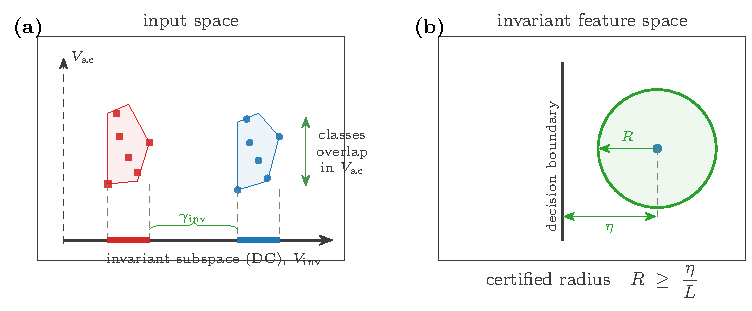
\includegraphics[width=0.86\linewidth]{concept.pdf}
  \caption{The two quantities the paper separates. \textbf{(a)}~Imposing shift-invariance projects each
  class onto the invariant subspace $\Vinv$ (the DC direction); the classes can overlap in the
  anti-invariant part $V_{\mathrm{ac}}$, and the surviving discriminative margin $\gamma_{\mathrm{inv}}$
  is their separation along the invariant direction (Theorem~\ref{thm:A}). \textbf{(b)}~Robustness is a
  distance: the certified radius satisfies $R\ge\etaL$, the margin over the sensitivity.}
  \label{fig:concept}
\end{figure}

%======================================================================
\section{Setup and definitions}\label{sec:prelim}
%======================================================================
We study classifiers $f:\R^\dd\to\R^K$ and the margin $M(x)=f_y(x)-\max_{j\neq y}f_j(x)$ at the correct
label $y$, which is positive exactly when $x$ is classified correctly. The \emph{robust radius} $r(x)$
is the smallest $\lVert\delta\rVert$ with $M(x+\delta)\le 0$; robust accuracy at budget $\epsilon$ is
the fraction of test points with $r(x)>\epsilon$, which we always measure with AutoAttack
\citep{croce2020reliable} and cross-check against a per-sample minimum-norm attack for the radius.
\emph{Shift-consistency} is the fraction of translations of $x$ that leave the top-1 label unchanged.

\paragraph{The threat-matched ratio and its shape.}
The per-image ratio is $M(x)/\lVert\grad_x M(x)\rVert_q$ with $q$ dual to the attack norm; the summary
$\etaL$ uses the means over correctly classified clean images. We also read the \emph{shape} of the
gradient through its anisotropy
\[
  A(x)=\frac{\lVert\grad_x M(x)\rVert_1}{\lVert\grad_x M(x)\rVert_2}\in[1,\sqrt\dd],
\]
which is near $1$ when the gradient is concentrated on a few coordinates and near $\sqrt\dd$ when it is
spread uniformly. Note $A=(\eta/L_2)/(\eta/L_1)$, so it is the same margin and gradient read as a ratio
of the two threat-matched ratios; like $\etaL$ it is gauge-free.

\paragraph{Gauge-freeness as an organizing principle.}
Because $f\mapsto cf$ scales $\eta$ and $L$ together, robustness attaches to the ratio, not to the
margin or the Lipschitz term alone; those two are individually gauge-dependent, so ``larger margin'' or
``smaller Lipschitz'' is well posed only once a scale is fixed. We anchor every robustness claim on the
gauge-invariant quantities $\etaL$, $A$, and the certified radius, and read any margin/Lipschitz split
at the training-fixed logit scale.

\paragraph{Three model families.} Our evidence spans three families, each answering a different
question. \emph{Small CIFAR, MNIST, and Fashion-MNIST classifiers and a PreActResNet-18}, where we build
capacity-matched architectures so that only the shift-invariance mechanism differs, isolate the
dissociation (\S\ref{sec:etaL}). \emph{Thirty adversarially trained CIFAR-10 models from RobustBench}, an
independent family we did not train, test whether the gradient's shape ranks robustness
(\S\ref{sec:aniso}). \emph{Sixteen frozen vision-language (CLIP) image encoders} (ten of them
adversarially robust) are where invariance is saturated (\S\ref{sec:saturation}) and where a per-image
analysis removes the adversarial-training confound (\S\ref{sec:etaL}).

%======================================================================
\section{Invariance is saturated and does not rank robustness}\label{sec:saturation}
%======================================================================
The invariance metric the anti-aliasing literature tracks cannot separate modern models. Across sixteen
frozen vision-language image encoders, robust and non-robust alike, shift-consistency ranges only from
$0.963$ to $0.988$: every modern encoder is already near-perfectly shift-consistent, so the metric has
no room to order them on any kind of robustness. Once clean accuracy is controlled it does not predict
common-corruption robustness either. The same squeeze appears on strong CNN backbones.

This has a direct empirical consequence, the dissociation defined above. In a
capacity-matched architectural dissection (four operators built to have identical parameter counts, so
only the shift-invariance mechanism differs), shift-consistency does not order adversarial robustness,
and under adversarial training it \emph{anti-predicts} it: the exactly shift-invariant operator has
perfect consistency and the \emph{lowest} robust accuracy. The threat-matched $\etaL$ orders robustness
instead. Table~\ref{tab:dissoc} previews the pattern that the next sections make precise across
settings.

\begin{table}[t]\centering\small
  \caption{The dissociation across settings. $\etaL$ orders robustness where shift-consistency does not.
  Values correlate with the robust radius (standard training) or threat-matched AutoAttack (adversarial
  training): Pearson for the CIFAR and ResNet grids, Spearman for the per-image CLIP result (within a
  fixed encoder).}
  \label{tab:dissoc}
  \begin{tabular}{lccc}
    \toprule
    setting & $\etaL$ vs robustness & shift-consistency vs robustness & reference \\
    \midrule
    CIFAR-10 classifiers (standard)   & $+0.998$ & uninformative ($-0.33$, n.s.) & \S\ref{sec:etaL} \\
    PreActResNet-18 (AT)              & $+0.91$ & anti-predicts ($-0.81$) & \S\ref{sec:etaL} \\
    Frozen CLIP encoders (per image)   & $+0.74$ to $+0.96$ & $+0.37$ to $\approx 0$ & \S\ref{sec:etaL} \\
    \bottomrule
  \end{tabular}
\end{table}

%======================================================================
\section{The ``invariance helps'' effect is a weak-attack artifact}\label{sec:weak}
%======================================================================
Reports that architectural invariance confers adversarial robustness without adversarial training are
measured with weak attacks. On every non-robust encoder, single-step FGSM reports $16$ to $61\%$ robust
accuracy, and AutoAttack erases it to zero (Figure~\ref{fig:weak}). Under FGSM the ``invariance helps''
ordering appears, a real trend; under AutoAttack there is no robustness left to order and the trend
disappears. This is the classic gradient-masking signature \citep{athalye}: a weak attack
overstates robustness, and the apparent correlation with invariance rides on that overstatement. We
confirm the same on CNNs: retraining the two operators reported to make invariance help
\citep{saha2024improving,wang2025bridging} under their own code and recipe, their advantage reproduces
under FGSM and vanishes under AutoAttack. We check for gradient masking throughout, and find none where
we make a positive $\etaL$ claim: AutoAttack robust accuracy stays at or below matched multi-step PGD in
every adversarially trained cell, and on the frozen encoders the parameter-free ensemble does not fall
below its APGD component.

\begin{figure}[t]\centering
  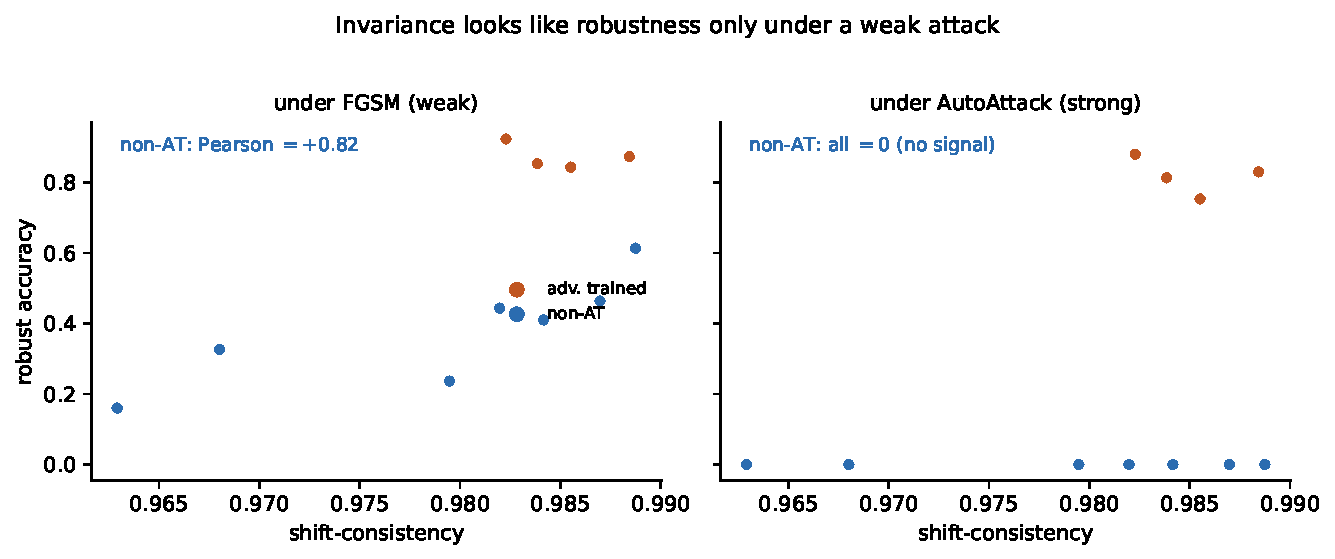
\includegraphics[width=0.6\linewidth]{fig3_weakattack.pdf}
  \caption{Same encoders and budget. Shift-consistency looks like it predicts robustness under FGSM
  (left) and predicts nothing under AutoAttack (right), because FGSM overstates the robustness of
  non-robust encoders that AutoAttack drives to zero.}
  \label{fig:weak}
\end{figure}

%======================================================================
\section{The margin-to-Lipschitz ratio predicts robustness}\label{sec:etaL}
%======================================================================
\paragraph{Theory: a two-sided bracket.}
The certificate $r\ge\etaL$ is the standard first-order lower bound. We complete it to a two-sided
bracket. Let $\alpha$ be a reachability slope: the slowest rate at which the margin can fall as one walks
from $x$ toward the boundary (a lower bound on that rate). Then
\[
  \etaL\;\le\;r\;\le\;\eta/\alpha,
\qquad\text{so}\qquad
  1\le \frac{r}{\etaL}\le \kappa:=\frac{L}{\alpha}.
\]
The gap is a local condition number $\kappa=L/\alpha$; when $\kappa$ is close to one, $\etaL$ is not
just a bound but tight, essentially the radius itself. The upper arm requires $\alpha$ to be certified
independently and to correspond to a genuine (transversal) boundary crossing, and we certify it in two
settings: for linear invariant features the two sides coincide exactly ($\kappa{=}1$,
$r=\eta/\lVert w\rVert$, recovering \citet{hein2017formal}), and for a radial power-spectrum surrogate,
whose reaching geometry is known a priori, the true radius lies strictly inside the bracket with
$\kappa\in[1.6,2.4]$. For a trained network $\alpha$ is not independently certified, so there the upper
arm is a \emph{conditional} converse, not a certified bound. This supplies the upper arm that the
margin-Lipschitz bound of \citet{tsuzuku2018lipschitz} leaves open, for feature families with a-priori
reachability. The gauge-freeness and the structural theory
behind $\eta$ (the invariant linear margin is the separation of the data projected onto the invariant
subspace, which recovers the $1/\sqrt\dd$ collapse of \citet{ge2021shift}) are in
Appendix~\ref{app:theory}.

\paragraph{Evidence across families.}
The same law holds from small CNNs to frozen foundation models.
\begin{itemize}[leftmargin=1.2em,itemsep=2pt]
\item \textbf{CIFAR-10, standard training.} Across a capacity-matched grid ($24$ runs over eight
arm-by-width cells), $\etaL$ orders the $\ell_2$ robust radius at Pearson $+0.998$; on the eight cell
means, controlling for clean accuracy, the partial is $+0.994$, while shift-consistency does not order
the radius (Pearson $-0.33$, $p=0.11$; partial $-0.59$, n.s.). This is a within-model tightness check,
since $\etaL$ lower-bounds each model's own radius; the cross-model and per-image results below are the
out-of-sample evidence.
\item \textbf{PreActResNet-18, adversarial training.} Over twelve architecture-by-width cells the
threat-matched $\eta/\lVert\grad M\rVert_1$ orders AutoAttack robustness at Pearson $+0.91$
($p<10^{-3}$), carrying robustness information beyond clean accuracy (partial correlation $+0.89$
controlling for clean accuracy); shift-consistency anti-predicts at $-0.81$ (partial $-0.82$). At
ImageNet-100 resolution, where clean accuracy is essentially constant across arms ($0.641$ to $0.649$),
the same threat-matched law holds at $+0.90$ while shift-consistency anti-predicts at $-0.87$, so the
prediction is not a restatement of clean accuracy. Controlling clean accuracy at the operator-arm level
(the four capacity-matched operators, eight arm-by-width cells) leaves the ordering intact: $\eta/L_1$
orders AutoAttack robustness at partial $+0.95$ and shift-consistency anti-predicts at $-0.86$.
\item \textbf{Frozen CLIP encoders, per image.} Within each of ten adversarially robust encoders, where
adversarial training cannot act as a confound, the per-image $\etaL$ orders the per-image adversarial
radius at Spearman $+0.74$ to $+0.96$, while per-image shift-consistency orders it from $+0.37$ down to
essentially zero, and the gap is significant in a paired test in every encoder (Figure~\ref{fig:perimg}).
This ordering is fine-grained, not a floor effect: on the hardened panel's thirteen robust encoders
($n{=}2600$) only $2.3\%$ of images sit at the radius floor, and excluding them leaves the pooled
per-image Spearman essentially unchanged ($+0.86\to+0.85$; every encoder survives individually).
\end{itemize}
Fitted without a held-out learnable-invariance operator, $\etaL$ predicts that operator's robustness out
of sample, and the same threat-matched law holds when we intervene on the training \emph{data} instead
of the architecture, through diffusion-augmented adversarial training (Appendix~\ref{app:extra}).

\begin{figure}[t]\centering
  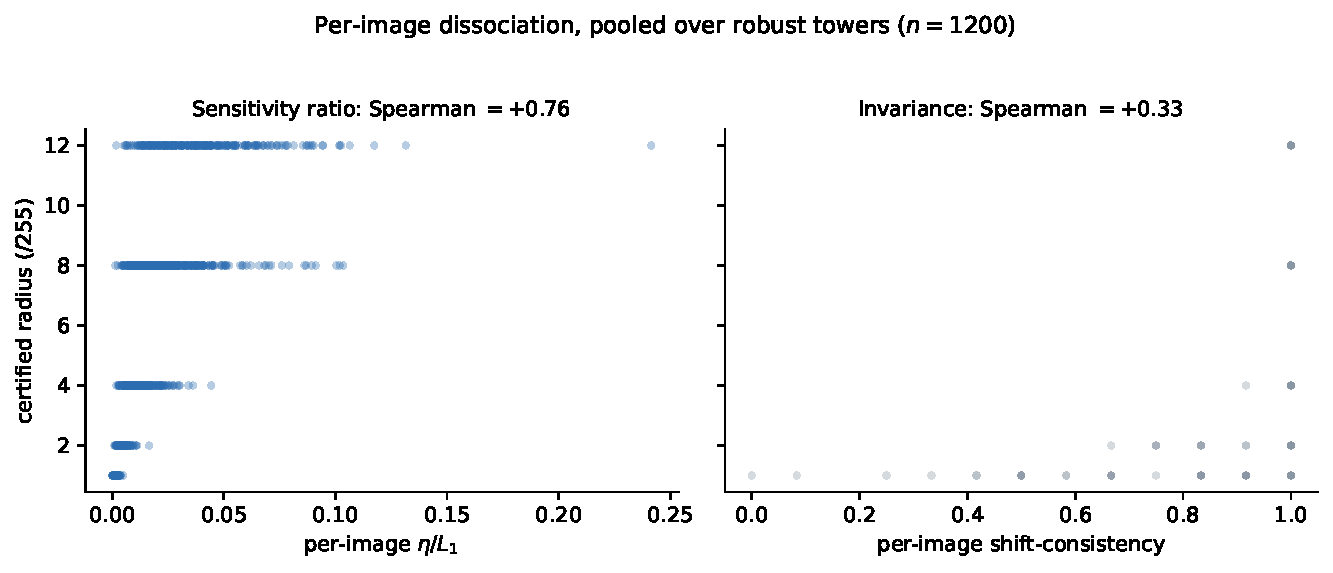
\includegraphics[width=0.72\linewidth]{fig2_perimage.pdf}
  \caption{Per image, pooled over the robust CLIP encoders ($n{=}1200$; each comparison is within one
  encoder, so adversarial training cannot confound it). The threat-matched ratio $\eta/L_1$ (left,
  Spearman $+0.76$) orders each image's certified radius; shift-consistency (right, $+0.33$) does not.
  Per-encoder ranges ($+0.74$ to $+0.96$ versus $+0.37$ to near zero) are in the text.}
  \label{fig:perimg}
\end{figure}

%======================================================================
\section{Detecting is not ranking: gradient shape and its mechanism}\label{sec:aniso}
%======================================================================
The ratio $\etaL$ cleanly \emph{separates} robust models from fragile ones, but \emph{across} the
already-robust models it no longer orders them: two encoders with the same $\etaL$ can differ in
robustness, and $\eta/L_1$ ranks the thirty robust RobustBench models only weakly
(Figure~\ref{fig:aniso}b). This is a different axis from the per-image ranking of \S\ref{sec:etaL}, which
holds \emph{within} a single encoder; here we compare \emph{across} robust models. The ratio uses the
\emph{size} of the gradient; ranking robust models needs its \emph{shape}.

\paragraph{Anisotropy ranks robust models.}
An $\ell_\infty$ attack pushes on every coordinate at once. If the margin's gradient is concentrated on
a few coordinates, most of the budget is wasted and the model holds; if it is spread over many, the
attack engages all of them. The anisotropy $A$ measures exactly this spread. Across thirty official
RobustBench CIFAR-10 $\ell_\infty$ models (a family independent of the CLIP encoders), lower $A$ means
more robust: Spearman$(A,\text{robust})=-0.79$ over the thirty models (bootstrap interval
$[-0.92,-0.56]$), which survives controlling for clean accuracy (partial $-0.77$) and for $\eta/L_1$
itself (partial $-0.65$). It also survives the natural capacity confound and the choice of attack:
against the models' \emph{official} RobustBench AutoAttack accuracy, partialling out clean accuracy
\emph{and} a model-size proxy jointly leaves $-0.69$ ($p{=}4\times10^{-5}$), and the ranking holds
\emph{within} one architecture family, ordering the twenty-two WideResNets at $-0.67$
($p{=}6\times10^{-4}$). And $A$ is not a free knob fit after the fact: added to $\eta/L_1$ it improves
leave-one-out prediction of held-out robustness by $30\%$ (rank correlation $+0.67\to+0.74$). Restricted
to the twenty-nine robust models the ranking is $-0.77$ (Figure~\ref{fig:aniso}a). The size $\eta/L_1$ detects robustness but ranks it only weakly
(Figure~\ref{fig:aniso}b). The same negative ranking appears within the robust CLIP encoders.

\begin{figure}[t]\centering
  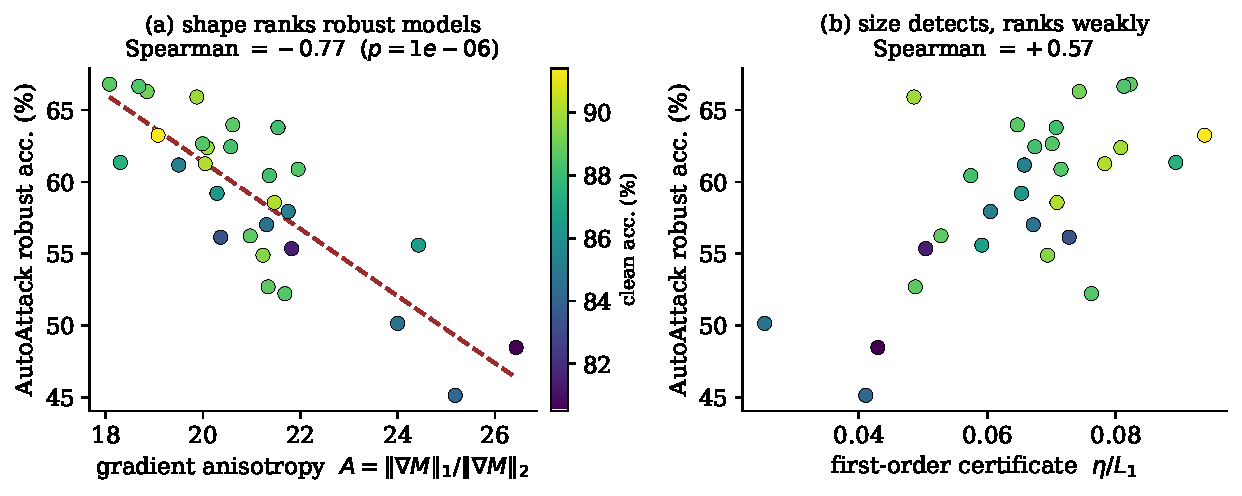
\includegraphics[width=0.82\linewidth]{robustbench_aniso.pdf}
  \caption{Thirty RobustBench CIFAR-10 models. \textbf{(a)} the gradient's shape $A$ ranks robustness
  (Spearman $-0.77$, surviving a clean-accuracy control); \textbf{(b)} the size $\eta/L_1$ detects
  robustness but ranks it only weakly.}
  \label{fig:aniso}
\end{figure}

\paragraph{The mechanism: an effective-dimension margin deficit.}
Why does spread hurt? The first-order estimate $\eta/L_1$ is only the leading term. A real attack also
harvests the gradient's variation across coordinates, and it collects more of that variation when the
gradient is spread over more coordinates. This shrinks the true radius below $\eta/L_1$ by a factor that
grows with the spread:
\begin{equation}
  r\;\approx\;\frac{\eta/L_1}{1+C\,A},
  \label{eq:deficit}
\end{equation}
with a model-level constant $C$. In a controlled model with the margin and the total gradient energy
held fixed and only the effective dimension varied, the true multi-step $\ell_\infty$ radius orders
perfectly against $A$ (Spearman $-1.0$), and the deficit scales as $\sqrt{\text{active dims}}=A$
(log-log slope $0.53$). The effect is \emph{transverse}, spread over the many coordinates, not the
curvature straight along the attack: we measured the on-direction curvature and it does \emph{not} rank
robustness, and $A$ does not track it, exactly as in the real encoders. So the curvature-regularization
account \citep{moosavi2019curvature} is not the ranking mechanism here.

\paragraph{Relation to prior work, and scope.}
The magnitude-versus-spread reading is the relaxation of \citet{simongabriel2019adversarial}, whose
dimension law assumes equal gradient variance per coordinate and so fixes $A\propto\sqrt\dd$; we let $A$
vary at fixed $\dd$ and find it tracks robustness. The nearest metric is the participation ratio of the
input gradient \citep{participation2025}, which equals $\dd/A^2$ up to normalization; it is used there to
\emph{detect} catastrophic overfitting during training, so our contribution is the cross-model ranking,
not the statistic itself. The synthetic model in Eq.~\ref{eq:deficit} is a
self-consistent stand-alone that assumes per-coordinate independence, not a derivation from the network;
the strong signal is between models, so $C$ is a model-level property. We therefore present the deficit
as a proposed mechanism, consistent with every control and refuting the curvature alternative, rather
than as a first-principles theorem. The law also generalizes to two low-dimensional families. On MNIST
and Fashion-MNIST a fixed-budget grid compresses $A$ into a narrow band and it does not rank, but
widening the range with an adversarial-training-strength sweep restores it, so the compression, not the
low input dimension, was the obstacle. Over twenty-four MNIST cells (with $A$ now spanning $[2.4,16.6]$)
$A$ ranks threat-matched $\ell_\infty$ robustness at the informative budgets, $-0.83$ ($\varepsilon{=}0.2$)
and $-0.89$ ($\varepsilon{=}0.3$) on MNIST (partial controlling clean accuracy $-0.75$ and $-0.74$), and
$-0.61$ ($\varepsilon{=}0.1$) to $-0.80$ ($\varepsilon{=}0.15$) over twenty-four Fashion-MNIST cells
(partial $-0.53$ and $-0.67$). Two caveats carry over: the sign is correct only in the training norm (in
the mismatched $\ell_2$ radius on MNIST $A$ takes the wrong sign, $+0.48$ raw, collapsing to $+0.10$ once
clean accuracy is controlled), and on this single-knob sweep $A$ is collinear with training strength
($\mathrm{Spearman}(A,\varepsilon)\approx-0.9$), so the cleaner cross-model evidence remains the diverse
RobustBench panel, where $A$ ranks robustness even after controlling for $\eta/L_1$
(Appendix~\ref{app:extra}).

%======================================================================
\section{Robust training re-couples margin and sensitivity}\label{sec:signflip}
%======================================================================
The two ingredients of $\etaL$ are coupled, and adversarial training changes how. In a standard model the
per-image margin and gradient size are anti-aligned: high-margin images sit in flatter regions with
\emph{smaller} gradients (within-model Spearman $\rho(M,\lVert\grad M\rVert_2)\approx-0.5$ in every one of
the twelve standard models), so margin and robustness reinforce. Adversarial training flips this to
positive ($\approx+0.5$ in every one of the twenty-four robust models): a robust model buys extra margin
partly by raising local sensitivity, so the margin-to-sensitivity ratio is self-limiting
(Figure~\ref{fig:signflip}). The per-image coupling flips sign, consistently across dozens of models.
This is why one ratio predicts robustness in both regimes: the margin and the gradient size, read
separately, are anti-aligned in standard models and aligned after robust training, and only their ratio
$\etaL$ tracks robustness through both. The same re-coupling explains why $\etaL$ is a diagnostic and not
a trainable target: because the ratio is scale-invariant its direct maximizer is a flat, zero-gradient score
(Lemma~\ref{lem:ratiodegen}), and first-order attempts to raise it collapse the margin
(Appendix~\ref{app:extra}).

\begin{figure}[t]\centering
  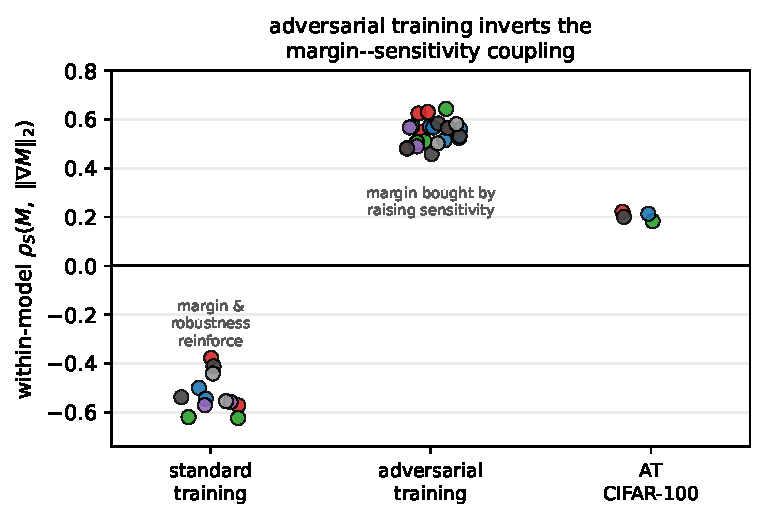
\includegraphics[width=0.7\linewidth]{resnet_persample_signflip.pdf}
  \caption{The within-model coupling between margin $M$ and input-gradient norm $\lVert\grad M\rVert_2$
  flips sign under adversarial training: negative under standard training (high-margin points are
  flatter) and positive after adversarial training (margin is bought by raising sensitivity), for every
  model, across the ResNet grid on CIFAR-10 and CIFAR-100.}
  \label{fig:signflip}
\end{figure}

%======================================================================
\section{Invariance saturates across modalities}\label{sec:crown}
%======================================================================
The saturation of \S\ref{sec:saturation} is not specific to pixel shifts. On zero-shot CLIP over
ImageNet-100 we lay out a two-by-two: two modalities (image, text) crossed with two perturbation types
over a semantically-null family, an average-case invariance and a worst-case adversarial version.
Images are shifted (average) or attacked with full targeted AutoAttack (worst case); prompts are reworded
into eleven curated meaning-preserving paraphrases (average, paraphrase-consistency PC) or scored by the
worst of them (worst case, adversarial-paraphrase accuracy $S_{\text{text}}$). The panel is seventeen
encoders: four non-robust, thirteen adversarially robust, including two Sim-CLIP towers and one
text-hardened tower (Figure~\ref{fig:crown}).

Both invariance cells saturate: shift-consistency is $0.977\pm0.009$ and paraphrase-consistency
$0.977\pm0.007$. Only the image-adversarial cell carries cross-encoder spread ($S=0.385\pm0.244$, range
$[0,0.69]$, twenty-eight times the shift-consistency spread), and the threat-matched $\eta/L_1$ predicts
it ($+0.80$, CI $[0.44,0.95]$; partial controlling clean accuracy $+0.82$; per image within the robust
encoders $+0.89$, $n{=}2600$), while the consistencies do not (shift $+0.21$, paraphrase $-0.30$, both
intervals spanning zero). The one place the clean two-by-two does not materialize is the text-adversarial
cell: the worst of eleven curated paraphrases is itself a mild perturbation, so $S_{\text{text}}$ stays
narrow ($0.896\pm0.029$, four times the paraphrase spread), and $\eta/L_1$, an image-side quantity, is
orthogonal to its residual variation once clean accuracy is controlled ($-0.54$ raw, partial $+0.01$, so
the raw anti-correlation is a clean-accuracy artifact). Paraphrase-consistency co-moves with
$S_{\text{text}}$ ($+0.98$), but that is average against worst case over the same narrow family. A single
text-hardened encoder, adversarially fine-tuned on the text tower, has the highest $S_{\text{text}}$ and
paraphrase-consistency in the panel despite a middling vision $\eta/L_1$, which places text robustness as
a separate axis raised by text training and not by the vision margin.

We sharpen the prompt channel with a prompt-conditioned variant. On nine encoders (three non-robust,
six robust) we condition both the margin and the image AutoAttack on each of six meaning-preserving
prompts and on their ensemble head (Figure~\ref{fig:crownpc}). Read this way, the prompt-conditioned
$\eta/L_1$ still orders robustness across all fifty-four $(\text{encoder},\text{prompt})$ cells
(Spearman $+0.79$; robust radius $+0.77$; cluster-bootstrap CI $[0.27,0.93]$), reproducing the
cross-encoder prediction under every prompt. Prompt invariance again does not buy robustness: the
ensemble head, which is maximally prompt-invariant, is no more robust than the mean single prompt
($\Delta S=-0.002$, CI $[-0.018,0.015]$; more robust in only three of nine encoders), and adversarial
examples transfer across prompts almost completely (mean $0.93$), so the adversarial direction is
essentially prompt-independent. Consistent with saturation, rewording barely moves the margin within an
encoder (coefficient of variation $1.3\%$ in $\eta/L_1$), so this sharpens the between-encoder
prediction rather than adding a within-model dissociation; the attack here is a uniform APGD-CE upper
bound, which preserves the cross-cell ordering the correlations use.

Two things follow. The saturation of invariance metrics is modality-general: textual paraphrase
invariance is as saturated as visual shift invariance, and no more predictive of adversarial robustness.
And the margin diagnostic is modality-specific: $\eta/L_1$ read on the image tower governs the
image-adversarial axis, while a wide text-adversarial axis, if one is wanted, needs a stronger textual
perturbation than a small curated paraphrase set supplies.

\begin{figure}[t]\centering
  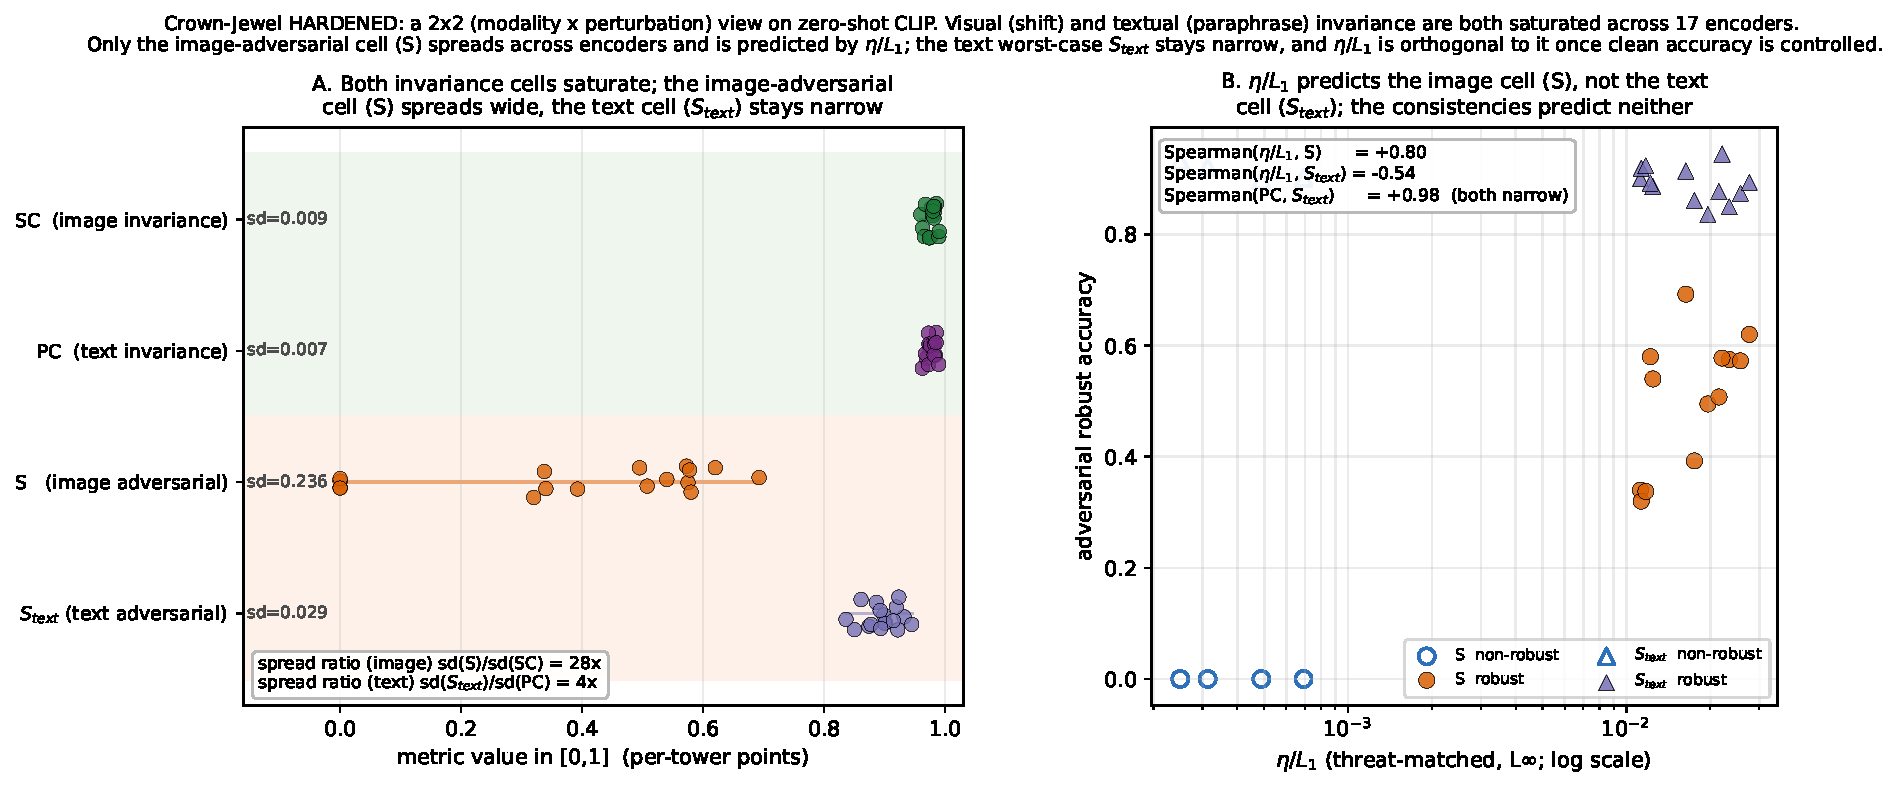
\includegraphics[width=0.99\linewidth]{crownjewel_hardened.pdf}
  \caption{Zero-shot CLIP, ImageNet-100, seventeen encoders, full targeted AutoAttack. \textbf{(a)}~both
  invariance cells (shift-consistency, paraphrase-consistency) saturate near $1$; the image-adversarial
  cell $S$ spreads widely while the text-adversarial cell $S_{\text{text}}$ (worst of eleven paraphrases)
  stays narrow. \textbf{(b)}~$\eta/L_1$ orders the image-adversarial cell ($+0.80$) but not the text cell
  ($-0.54$ raw, and zero after controlling for clean accuracy), and neither consistency orders either.
  The continuous $\ell_\infty$ image attack and the discrete paraphrase set are both worst cases over a
  semantically-null family; the small paraphrase set is the milder perturbation.}
  \label{fig:crown}
\end{figure}

\begin{figure}[t]\centering
  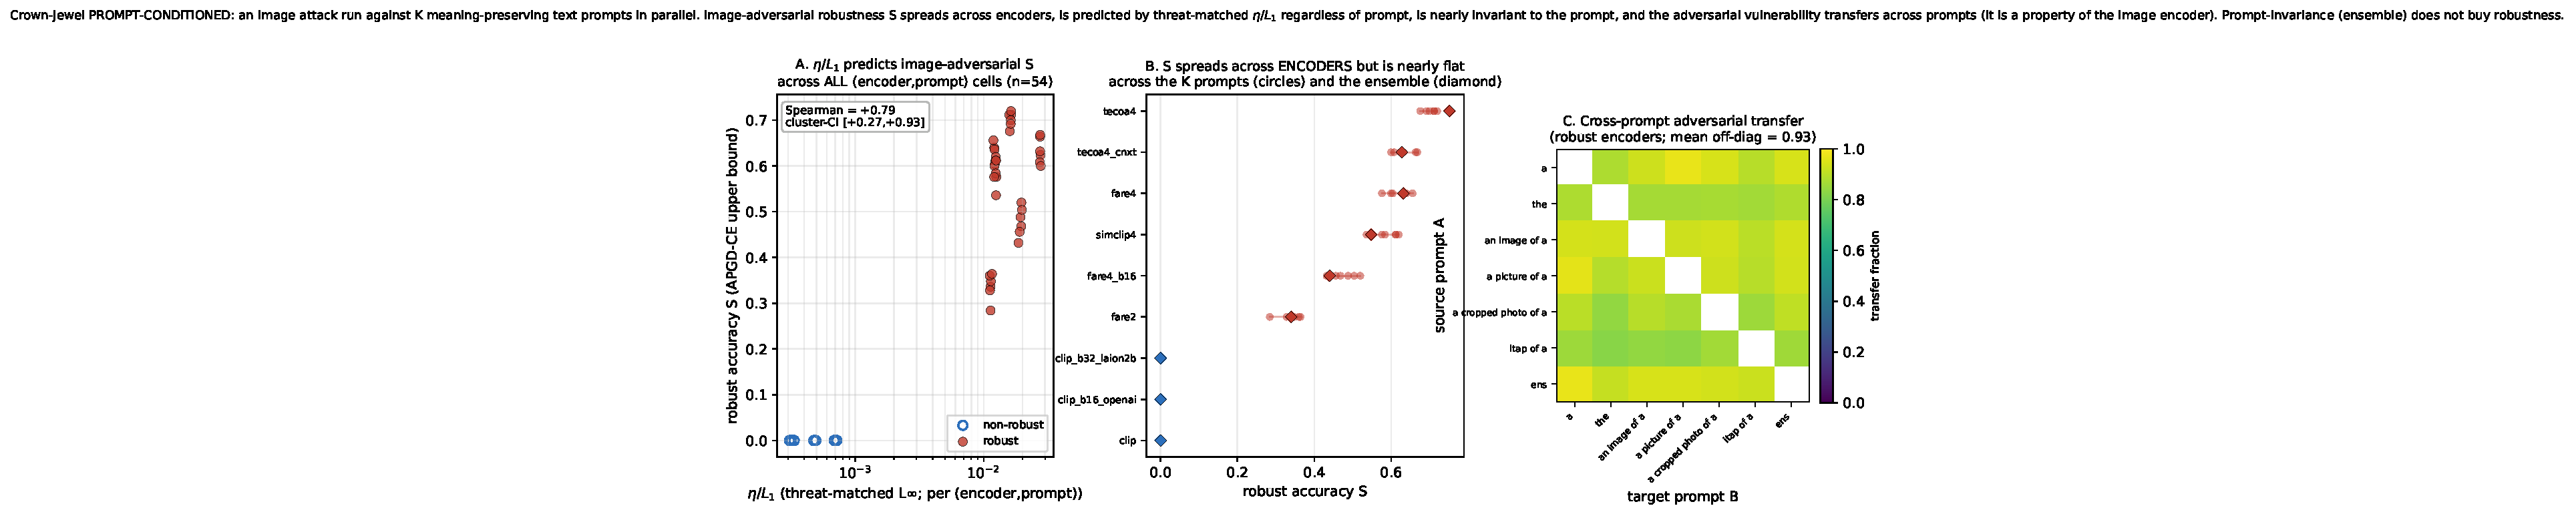
\includegraphics[width=0.94\linewidth]{crownjewel_promptcond.pdf}
  \caption{Prompt-conditioned check: nine CLIP encoders (three non-robust, six robust), six
  meaning-preserving prompts plus their ensemble, with the margin and the image AutoAttack conditioned on
  each prompt ($S$ is a uniform APGD-CE upper bound). \textbf{(A)}~the prompt-conditioned $\eta/L_1$ orders
  the image-adversarial $S$ across all $(\text{encoder},\text{prompt})$ cells ($+0.79$). \textbf{(B)}~$S$
  spreads across encoders but is nearly flat across the six prompts (circles) and the prompt-invariant
  ensemble (diamond), so prompt invariance does not buy robustness. \textbf{(C)}~adversarial examples
  transfer across prompts (mean off-diagonal $0.93$), so the vulnerability is a property of the image
  encoder, not the prompt. A prompt-channel confirmation of the modality-general saturation, not a
  separate within-model effect.}
  \label{fig:crownpc}
\end{figure}

%======================================================================
\section{Related work}\label{sec:related}
%======================================================================
\textbf{Invariance and robustness.} \citet{ge2021shift} give the trade-off on single-orbit data;
\citet{kamath2021canwehaveitall,tramer2019multiple} prove tensions between geometric and adversarial
robustness; the anti-aliasing line \citep{zhang2019making,grabinski2022aliasing,saha2024improving},
truly shift-invariant designs \citep{chaman2021truly}, and the equivariance line \citep{wang2025bridging}
report the opposite sign. We read these as positions on the threat-matched $\etaL$ axis: Ge's collapse
and the trade-off results are the small-margin corner, where invariance costs margin and $\etaL$ falls,
while the ``helps'' reports are a weak-attack reading that does not survive AutoAttack rather than a third
regime. We demonstrate the weak-attack reading directly for the two operators we retrain
(\S\ref{sec:weak}) and offer the $\etaL$-axis account as a unifying narrative for the broader line.
\textbf{Attack-free robustness estimates.} CLEVER \citep{clever}, the generative GREAT Score
\citep{greatscore}, and margin-Lipschitz certificates \citep{hein2017formal,tsuzuku2018lipschitz}
estimate a radius; we make the estimate gauge-free, threat-matched, and two-sided, and add the anisotropy
refinement for ranking robust models. Certified defenses such as randomized smoothing
\citep{cohen2019certified} also return a radius, but through a smoothed classifier and sampling; $\etaL$
is complementary, a first-order read of the base model that needs no smoothing and no attack.
\textbf{Gradient geometry.} \citet{simongabriel2019adversarial} tie vulnerability to gradient norm and
dimension under equal per-coordinate variance; we relax that assumption. \citet{moosavi2019curvature}
regularize curvature for robustness; we show on-direction curvature does not rank robust models and the
transverse effective-dimension deficit does. The gradient participation ratio \citep{participation2025}
is used for overfitting detection, not cross-model ranking.

%======================================================================
\section{Limitations and discussion}\label{sec:disc}
%======================================================================
The tower-level CLIP correlation rests on a small number of robust encoders, so the per-image result is
the load-bearing one; the hardened multimodal benchmark (\S\ref{sec:crown}) expands the panel and uses
full AutoAttack. Several tower-level correlations rest on $n{=}17$ to $30$ with wide intervals and no
family-wise correction; we treat these as suggestive and lean on the large-$n$ per-image (thousands of
images) and RobustBench analyses for the load-bearing claims. The prompt-conditioned panel
(\S\ref{sec:crown}) scores robustness with a uniform APGD-CE upper bound rather than full targeted
AutoAttack; applied identically to every cell it can only lower $S$ and preserves the cross-cell ordering
the correlation uses. The deficit law of Eq.~\ref{eq:deficit} is a proposed, well-controlled mechanism rather
than a network-level theorem, and the ranking it drives is range-dependent: it needs a wide robustness
axis, which on low-dimensional families appears only once a training-strength sweep opens it. Finally
$\etaL$ is a diagnostic to read off a trained model, not a target to train toward. Within those limits, one idea, the margin relative to the
sensitivity, unifies a split literature, corrects a common evaluation mistake, and turns a vague
intuition about invariance into something measurable: invariance is not robustness, the margin relative
to the sensitivity is, its shape is what separates the strong models, and the saturation of invariance
carries from pixel shifts to text.

\paragraph{Reproducibility and ethics.} All quantities are computed with released attack code
(AutoAttack, a minimum-norm attack) on standard benchmarks; the contribution is diagnostic and
defensive, introducing no new attack. Code, configurations, and per-sample outputs are released.

\bibliographystyle{plainnat}
\bibliography{references}

\appendix

%======================================================================
% appendix_full.tex
% Maximally-detailed technical-report-depth appendix for the combined
% main-track paper. Meant to be \input at the \appendix point of main.tex.
% All proofs and tables are ported from paper/report/main.tex and
% paper/report/theory_full_checked_v2.tex, and every experimental number
% is traced to a source file (stated under each table). No number is
% invented or changed. See APPENDIX_PORT_NOTES.md for provenance and flags.
%
% Macros this file uses that are NOT in the combined main.tex preamble
% (move these to the preamble; they are defined here so the file compiles
% standalone in the test wrapper):
%   \Vac  \Sep  \Z  \E  \one  \Piinv  \sign  \conv  \dist  \Lip  \Orb
% They are guarded with \providecommand so re-definition is harmless.
%======================================================================

\providecommand{\Z}{\mathbb{Z}}
\providecommand{\E}{\mathbb{E}}
\providecommand{\Vac}{V_{\mathrm{ac}}}
\providecommand{\Sep}{\mathrm{Sep}}
\providecommand{\one}{\mathbf 1}
\providecommand{\Piinv}{\Pi_{\mathrm{inv}}}
\providecommand{\sign}{\mathrm{sign}}
\providecommand{\conv}{\operatorname{conv}}
\providecommand{\dist}{\operatorname{dist}}
\providecommand{\Lip}{\operatorname{Lip}}
\providecommand{\Orb}{\mathcal O}

%======================================================================
\section{Full structural and optimization theory}\label{app:theory}
%======================================================================
This appendix gives, in full, the proofs the main text states or sketches, and
the supporting structural results. It is self-contained: \S\ref{app:ft-setup}
fixes notation, \S\ref{app:ft-margin}--\S\ref{app:ft-lazy} prove the six
load-bearing results in the order announced in the main body. Where the main
text scopes a claim as proposed or conditional (the effective-dimension deficit
of \S\ref{sec:aniso}, the rich-regime KKT conjecture of the optimization
discussion), that scoping is preserved verbatim here.

\subsection{Setup and standing notation}\label{app:ft-setup}
We work with one-dimensional signals $x\in\R^{\dd}$; the two-dimensional case
replaces $\Z_{\dd}$ by $\Z_{d_1}\times\Z_{d_2}$ and the cyclic discrete Fourier
transform (DFT) by its two-dimensional analogue, without change to any
statement. The cyclic group $G=\Z_{\dd}$ acts by the circular shift
$(S_sx)_i=x_{(i-s)\bmod\dd}$; each $S_s$ is an orthogonal permutation. The
\emph{orbit} of $x$ is $\Orb(x)=\{S_sx\}_{s\in G}$, and a class set is
\emph{orbit-closed} if it is closed under all shifts. Let
$\Vinv=\{v:S_sv=v\ \forall s\}$ and $\Vac=\Vinv^{\perp}$. The orthogonal
projector onto $\Vinv$ is $\Piinv=\tfrac1\dd\one\one^\top=ee^\top$ with
$e=\dd^{-1/2}\one$, so $\Vinv=\mathrm{span}(\one)$ is the constant (DC,
zero-frequency) line and $\Vac=\{v:\sum_iv_i=0\}$ is its zero-mean (AC)
complement. Write $\fdc(x)=e^\top x=\dd^{-1/2}\sum_ix_i$ for the unit DC
functional. With the unitary DFT $\hat x_k=\dd^{-1/2}\sum_jx_je^{-2\pi ijk/\dd}$
and $\omega=e^{2\pi i/\dd}$, a shift multiplies coefficient $k$ by the unit phase
$\omega^{sk}$, so $|\hat x_k|^2$ is shift-invariant.

For a score $f$ correct on $(x,y)$, the $\ell_p$ robust radius is
$r_p(f,x)=\inf\{\lVert\delta\rVert_p:\ \sign f(x+\delta)\neq y\}$; for a linear
score $w^\top x+b$ with $yf(x)>0$ this equals $y(w^\top x+b)/\lVert w\rVert_q$
($q$ dual to $p$). The margin at the correct label is
$M(x)=f_y(x)-\max_{j\neq y}f_j(x)$, positive exactly when $x$ is correct;
$\eta=\E[M]$ and $L=\E\lVert\grad M\rVert_q$ are the dataset means on correctly
classified clean points. For finite sets $A,B$ write the hard-margin separation
$\Sep(A,B):=\tfrac12\dist(\conv A,\conv B)$, zero when the hulls intersect. All
statements match the combined main text's notation and environments.

\begin{lemma}[Fixed subspace for cyclic shifts]\label{lem:cyclic-fixed}
For the cyclic shift action on $\R^\dd$,
$\Vinv=\mathrm{span}(\one)$, $\Piinv=\dd^{-1}\one\one^\top=ee^\top$, and
$\Vac=\{v:\one^\top v=0\}$. The shifts are simultaneously diagonalized by the
DFT, $FS_sF^{*}=\mathrm{diag}(\omega^{sk})_{k=0}^{\dd-1}$, each eigenvalue of
modulus one, so $|\widehat{S_sx}_k|^2=|\hat x_k|^2$ for every $k$.
\end{lemma}
\begin{proof}
If $v\in\Vinv$ then $S_1v=v$ reads $v_i=v_{i-1}$ modulo $\dd$, so all
coordinates are equal and $v\in\mathrm{span}(\one)$; conversely every constant
vector is fixed by every $S_s$. The orthogonal projector onto $\mathrm{span}(\one)$
is $\one\one^\top/\lVert\one\rVert_2^2=\dd^{-1}\one\one^\top=ee^\top$, with
complement $\{v:\one^\top v=0\}$. Every $S_s$ is a circulant permutation, hence
diagonalized by the DFT; its eigenvalues have modulus one, so shifting changes
only Fourier phases and preserves each $|\hat x_k|^2$.
\end{proof}

\subsection{Result 1: the invariant linear margin equals projection separation}
\label{app:ft-margin}
We restate Theorem~\ref{thm:A} of the main text identically, prove it in full
(reduction to one-dimensional DC thresholding; max-margin equals half the
inter-interval distance; the $\pm\one/\sqrt\dd$ direction; recovery of the Ge
$1/\sqrt\dd$ collapse), and give the finite-group generalization.

\begin{theorem}[Invariant linear margin equals projection separation; restated]
\label{thm:A}
A linear score $g(x)=w^\top x+b$ is shift-invariant for all $x$ if and only if
$w=c\one$. Consequently, for any finite separable classes $X_+,X_-$, the
invariant $\ell_2$ max-margin equals the separation of the DC-projected data,
\[
\gamma_{\mathrm{inv}}=\tfrac12\,\dist(I_+,I_-)
=\tfrac12\,\dist\big(\conv\Piinv X_+,\ \conv\Piinv X_-\big),
\]
where $I_\pm=[\min_{x\in X_\pm}\fdc(x),\ \max_{x\in X_\pm}\fdc(x)]$, with
maximizing direction $\pm\one/\sqrt\dd$ oriented toward the positive class. This
holds for any finite separable dataset and does not require orbit-closure; when the
DC-projected intervals $I_+,I_-$ overlap the formula gives $\gamma_{\mathrm{inv}}=0$,
i.e.\ full-space separability does not imply the invariant problem is separable.
\end{theorem}
\begin{proof}
\emph{Characterization of invariant normals.} Invariance of $g$ under every
shift means $w^\top S_sx=w^\top x$ for all $x,s$, i.e.\ $(S_{-s}w-w)^\top x=0$
for all $x$, hence $S_{-s}w=w$ for all $s$. The only vectors fixed by every
cyclic shift are the constants (Lemma~\ref{lem:cyclic-fixed}), so
$w\in\Vinv=\mathrm{span}(\one)$, i.e.\ $w=c\one$; conversely every $c\one$ gives
an invariant score.

\emph{Reduction to one-dimensional DC thresholding.} With $w=c\one$ the score
depends on $x$ only through $\fdc(x)=\one^\top x/\sqrt\dd$, because
$w^\top x=c\,\one^\top x=c\sqrt\dd\,\fdc(x)$. Thus the data reduce to their
scalar DC values and the classes to the intervals
$I_\pm=[\min_{X_\pm}\fdc,\max_{X_\pm}\fdc]$ on the line $\mathrm{span}(e)$.

\emph{Max-margin on the line.} The maximum-margin separator of two point sets on
a line places the threshold midway in the gap between their convex hulls (here
the two intervals $I_\pm$); its geometric margin is half the distance between
the intervals, $\gamma_{\mathrm{inv}}=\tfrac12\dist(I_+,I_-)$. Concretely, if
$I_+$ lies to the right of $I_-$ the optimal unit normal is $+e=+\one/\sqrt\dd$
and $\gamma_{\mathrm{inv}}=\tfrac12(\min_{X_+}\fdc-\max_{X_-}\fdc)$; if $I_-$
lies to the right the normal is $-e$; and when the intervals overlap the
separation, hence the invariant margin, is $0$. Identifying the projected line
with $\mathrm{span}(\one)$ isometrically gives the convex-hull form
$\tfrac12\dist(\conv\Piinv X_+,\conv\Piinv X_-)$.
\end{proof}

\begin{corollary}[Recovery of the Ge $1/\sqrt\dd$ collapse]\label{cor:ge-recover}
For the single white/black dot $x_+=e_j$, $x_-=-e_j$ one has
$\fdc(\pm e_j)=\pm1/\sqrt\dd$, so Theorem~\ref{thm:A} gives
$\gamma_{\mathrm{inv}}=1/\sqrt\dd$ (half-gap convention; the full DC gap is
$2/\sqrt\dd$), the collapse of \citet{ge2021shift}. The unconstrained max-margin
of the two unshifted points $\{e_j\},\{-e_j\}$ is $1$, but on the orbit-closed
dataset $\Orb(e_j)$ versus $\Orb(-e_j)$ the unconstrained linear max-margin is
itself $1/\sqrt\dd$, so the $1$-versus-$1/\sqrt\dd$ contrast is a property of the
two-image protocol, not of invariance alone.
\end{corollary}
\begin{proof}
$\fdc(\pm e_j)=e^\top(\pm e_j)=\pm1/\sqrt\dd$ gives the invariant margin
directly. On $\Orb(e_j)$ vs $\Orb(-e_j)$ every positive basis vector must be
classified positive and every negative one negative by a single hyperplane; the
symmetric max-margin solution is $w\propto\one$ with margin $1/\sqrt\dd$, so the
unconstrained and invariant margins coincide there.
\end{proof}

\begin{proposition}[General finite-group invariant margin]\label{prop:finite-group-app}
Let a finite group $G$ act orthogonally on $\R^\dd$ by matrices $\{R_g\}$, with
fixed subspace $V^G=\{v:R_gv=v\ \forall g\}$ and group-average projector
$P_G=\tfrac1{|G|}\sum_{g}R_g$. A linear score $w^\top x+b$ is exactly
$G$-invariant if and only if $w\in V^G$, and the maximum invariant $\ell_2$
margin for finite separable classes is
$\gamma_{\mathrm{inv}}=\tfrac12\dist(\conv P_GX_+,\conv P_GX_-)$.
Theorem~\ref{thm:A} is the cyclic case $P_G=\Piinv$.
\end{proposition}
\begin{proof}
$P_G$ is the orthogonal projector onto $V^G$: group closure gives
$P_G^2=|G|^{-2}\sum_{g,h}R_gR_h=|G|^{-1}\sum_kR_k=P_G$; each $R_g$ orthogonal
gives $R_g^\top=R_{g^{-1}}$ and $P_G^\top=P_G$; its range is exactly $V^G$.
Invariance of $w^\top x$ for all $x$ is equivalent to $R_g^\top w=w$ for all $g$,
hence (as $G$ is a group) to $R_gw=w$, i.e.\ $w\in V^G$. For $w\in V^G$ we have
$w=P_Gw$, so $w^\top x=w^\top P_Gx$: every invariant linear classifier on
$X_\pm$ is an ordinary linear classifier on the projected sets $P_GX_\pm$, with
the same normal and signed margins. The maximum unit-normal margin separating
two finite sets $A,B$ equals $\tfrac12\dist(\conv A,\conv B)$, attained by the
unit vector along the closest-points segment of the hulls: if every point of
$A,B$ is at signed distance $\ge\gamma$ from a unit-normal hyperplane, so is
every convex combination, so the hulls are at distance $\ge2\gamma$; the segment
midpoint realizes it. Apply this to $A=P_GX_+$, $B=P_GX_-$.
\end{proof}

\begin{corollary}[Projection cannot increase the linear max-margin]\label{cor:proj-mono}
With $\gamma_{\mathrm{full}}=\tfrac12\dist(\conv X_+,\conv X_-)$ and
$\gamma_{\mathrm{inv}}$ as above, $\gamma_{\mathrm{inv}}\le\gamma_{\mathrm{full}}$,
because orthogonal projectors are non-expansive:
$\lVert P_Gu-P_Gv\rVert_2\le\lVert u-v\rVert_2$, so taking the infimum over the
hulls preserves the inequality.
\end{corollary}

\subsection{Result 2: the two-sided bracket (a conditional converse)}
\label{app:ft-bracket}
We restate Proposition~\ref{prop:sandwich} of the main text and give the full
proof, with the explicit reaching-path and co-Lipschitz$(\alpha)$ hypotheses,
the exact linear case $\kappa=1$ \citep{hein2017formal}, the $t^{2n+1}$
large-$\kappa$ counterexample, and the note that it completes the missing upper
arm of \citet{tsuzuku2018lipschitz}.

\begin{proposition}[Two-sided bracket; restated]\label{prop:sandwich}
Let $g$ be continuous and $L$-Lipschitz in $\ell_2$ on a convex set $S$
containing $x$, its nearest boundary point, and the path $\gamma$ below, correct
at $x$ with margin $\eta=y\,g(x)>0$, and write $\mathcal B=\{z:g(z)=0\}$.
\emph{(Lower arm)} $r_2(g,x)\ge\eta/L$. \emph{(Upper arm)} if there is a
continuous path $\gamma:[0,T]\to S$ with $\gamma(0)=x$, $g(\gamma(T))=0$, and a
co-Lipschitz (lower-Lipschitz) bound
$|g(\gamma(t))-g(x)|\ge\alpha\lVert\gamma(t)-x\rVert_2$ up to the first boundary
hit, then $r_2(g,x)\le\eta/\alpha$, and necessarily $\alpha\le L$. Hence
\[
\frac{\eta}{L}\ \le\ r_2(g,x)\ \le\ \frac{\eta}{\alpha},\qquad
\kappa:=\frac{L}{\alpha}\ge1,
\]
so $\etaL$ determines the robust radius up to the local bi-Lipschitz condition
number $\kappa$; the certificate is exact ($r_2=\eta/L$) iff $\kappa=1$.
\end{proposition}
\begin{proof}
Convexity of $S$ keeps the relevant segments inside $S$, so the local Lipschitz
and co-Lipschitz constants apply along them.

\emph{Lower arm.} For any $\delta$ with $\lVert\delta\rVert_2<\eta/L$ the
Lipschitz bound gives $|g(x+\delta)-g(x)|\le L\lVert\delta\rVert_2<\eta=|g(x)|$,
so $g(x+\delta)$ keeps the sign of $g(x)$ and no perturbation below $\eta/L$
flips the label; hence $r_2\ge\eta/L$. This is the standard Lipschitz--margin
certificate \citep{hein2017formal,tsuzuku2018lipschitz}.

\emph{Upper arm.} At $t=T$, $g(\gamma(T))=0$ and $|g(x)|=\eta$, so
$\eta=|g(x)-g(\gamma(T))|\ge\alpha\lVert\gamma(T)-x\rVert_2$, giving
$\lVert\gamma(T)-x\rVert_2\le\eta/\alpha$. Provided $\gamma(T)$ is a \emph{transversal} crossing---$g$
changes sign there, rather than merely touching zero tangentially---the
perturbation $\delta=\gamma(T)-x$ is label-flipping and
$r_2\le\lVert\gamma(T)-x\rVert_2\le\eta/\alpha$. Transversality is a genuine
hypothesis: a tangential zero (e.g.\ $g(\gamma(t))=(t-1)^2\eta$) satisfies the
co-Lipschitz bound yet does not flip the label, so it cannot be dropped.

\emph{$\alpha\le L$.} As $g(\gamma(T))=0\neq g(x)$ we have $\gamma(T)\neq x$, and
the same secant obeys
$\alpha\lVert\gamma(T)-x\rVert_2\le|g(\gamma(T))-g(x)|\le L\lVert\gamma(T)-x\rVert_2$,
so $\alpha\le L$ and $\kappa\ge1$. Combining the arms gives the bracket, tight
iff $\kappa=1$. The upper arm is informative only when $\alpha$ is certified
independently of $r_2$: taking $\alpha$ as the secant slope of the minimal path
itself makes $r_2=\eta/\alpha$ a tautology, whereas the linear case and the
power-spectrum surrogate below fix $\alpha$ from the feature structure.
\end{proof}

\begin{corollary}[Linear invariant features: the converse is exact]\label{cor:linear-exact-app}
If $g(x)=w^\top x+b$ with $w\in\Vinv$ (so $g$ reads $x$ only through $\fdc$),
then along the straight path $\gamma(t)=x-t\,w/\lVert w\rVert_2$ one has
$|g(z)-g(x)|=|w^\top(z-x)|\le\lVert w\rVert_2\lVert z-x\rVert_2$ with equality
along $\pm w$, so $L=\alpha=\lVert w\rVert_2$, $\kappa=1$, and the boundary is
reached at distance $\eta/\lVert w\rVert_2$: the exact point-to-hyperplane
radius $r_2=\eta/\lVert w\rVert_2$ of \citet{hein2017formal}.
\end{corollary}

\begin{remark}[The large-$\kappa$ counterexample: $t^{2n+1}$]\label{rem:tpow-app}
There is no \emph{universal} converse. For the shift-invariant scalar feature
$\Psi_n(x)=t^{2n+1}$ with $t=\fdc(x)$, and points $x_+=e$, $x_-=-e$, the signed
feature margin is $\eta=1$. On the segment $\{te:t\in[-1,1]\}$ the Lipschitz
constant is $L_n=\max_{|t|\le1}(2n+1)t^{2n}=2n+1$, so the certificate gives
$\eta/L_n=1/(2n+1)$. But the boundary is $t=0$, reached from $e$ at Euclidean
distance $1$ (perturbations in $\Vac$ do not change $t$), so $r_2=1$ and
$r_2/(\eta/L_n)=2n+1\to\infty$. In the bracket language this is the large-$\kappa$
end: the straight DC path has secant slope $\alpha=1$, the upper Lipschitz is
$L=2n+1$, so $\kappa=2n+1$ and the bracket $[1/(2n+1),\,1]$ correctly contains
$r_2=1$ at its $\eta/\alpha$ end. The failure of a universal converse is exactly
the unboundedness of $\kappa$ over the model class, not the absence of a bracket
for a fixed model.
\end{remark}

\begin{remark}[Completing the Tsuzuku chain]\label{rem:tsuzuku-app}
\citet{tsuzuku2018lipschitz} (their Eq.~5) bound $r_2$ only from below through
successively tighter Lipschitz constants and state the top inequality
(certificate $\le$ true radius) cannot be guaranteed, measuring it empirically as
a $1.8$--$2.4\times$ gap. The upper arm $r_2\le\eta/\alpha$ of
Proposition~\ref{prop:sandwich} is the matching arm that turns their
one-sided certificate into a two-sided bracket. It is deterministic and tied to a
single fixed classifier, its looseness controlled by the explicit $\kappa$
rather than, as in the randomized-smoothing converse of \citet{cohen2019certified},
by a worst case over classifiers. We verify numerically that the true radius lies
strictly inside the bracket with $\kappa\in[1.6,2.4]$ for the power-spectrum
surrogate.
\end{remark}

For completeness we record the certifiable upper arm for the quadratic-invariant
class, where the reaching path, feature co-Lipschitz constant, and head slope are
all known a priori, so the bracket is genuinely two-sided (not tautological).

\begin{lemma}[Radial co-Lipschitz bound for the power spectrum]\label{lem:ps-colip-app}
Let $\Psi(x)=(|\hat x_k|^2)_k$ with the unitary DFT, and for $r_0,\sigma_0>0$ let
$\mathcal C(r_0,\sigma_0,B)=\{x:r_0\le\lVert x\rVert_2\le B,\ \lVert\Psi(x/\lVert x\rVert_2)\rVert_2\ge\sigma_0\}$.
For $x\in\mathcal C(r_0,\sigma_0,B)$ and $t\in[0,1]$,
$\lVert\Psi(x)-\Psi(tx)\rVert_2\ge r_0\sigma_0\lVert x-tx\rVert_2$.
\end{lemma}
\begin{proof}
Two-homogeneity gives $\Psi(tx)=t^2\Psi(x)$, so
$\lVert\Psi(x)-\Psi(tx)\rVert_2=(1-t^2)\lVert\Psi(x)\rVert_2$ while
$\lVert x-tx\rVert_2=(1-t)\lVert x\rVert_2$; the ratio is
$(1+t)\lVert\Psi(x)\rVert_2/\lVert x\rVert_2\ge\lVert x\rVert_2\lVert\Psi(x/\lVert x\rVert_2)\rVert_2\ge r_0\sigma_0$
on the cone, using $\Psi(x)=\lVert x\rVert_2^2\Psi(x/\lVert x\rVert_2)$ and
$1+t\ge1$.
\end{proof}

\begin{proposition}[Certifiable bracket for radial power-spectrum scores]\label{prop:ps-alpha-app}
Let $g=h\circ\Psi$ with $\Psi$ as above, $x\in\mathcal C(r_0,\sigma_0,B)$,
$g(x)>0$, $g(0)<0$; by continuity there is $t_\star\in(0,1)$ with
$g(t_\star x)=0$, set $z=t_\star x$. If
$h(\Psi(x))-h(\Psi(z))\ge h_-\lVert\Psi(x)-\Psi(z)\rVert_2$ for some $h_->0$,
then $r_2(x)\le g(x)/(h_-r_0\sigma_0)$. If in addition $h$ is $h_+$-Lipschitz on
$\Psi(B_2(0,B'))$ with $B'$ large enough that the certified neighborhood of $x$
stays in the ball, then
\[
\frac{g(x)}{2B'h_+}\ \le\ r_2(x)\ \le\ \frac{g(x)}{h_-r_0\sigma_0},
\qquad \kappa\le\frac{2B'h_+}{h_-\,r_0\sigma_0}.
\]
\end{proposition}
\begin{proof}
$\varphi(t)=g(tx)$ is continuous with $\varphi(0)<0<\varphi(1)$, giving
$t_\star$ and the boundary point $z=t_\star x$ on the explicit radial path.
Lemma~\ref{lem:ps-colip-app} and the head secant give
$g(x)=g(x)-g(z)\ge h_-r_0\sigma_0\lVert x-z\rVert_2$, so
$r_2(x)\le\lVert x-z\rVert_2\le g(x)/(h_-r_0\sigma_0)$. For the lower arm,
$|g(u)-g(v)|\le h_+\lVert\Psi(u)-\Psi(v)\rVert_2\le2B'h_+\lVert u-v\rVert_2$ on
the ball (Lemma~\ref{lem:ps-lip-app}), and the standard certificate applies. The
reaching path is the explicit radial path, the feature co-Lipschitz constant is
the explicit cone constant $r_0\sigma_0$, and $h_-$ is a property of the head on
a known feature segment, so all three are available before any attack is run: the
bracket is genuinely two-sided on the cone, not obtained by naming the unknown
secant slope of the true minimal path.
\end{proof}

\subsection{Result 3: scale-invariance of the ratio (gauge-freeness)}
\label{app:ft-scale}
We restate Lemma~\ref{lem:ratiodegen} of the main text, prove it, and record the
corollary that the direct maximizer is the constant classifier.

\begin{lemma}[Scale-invariance of the ratio; restated]\label{lem:ratiodegen}
The per-sample ratio $M(x)/\lVert\grad M(x)\rVert$ is invariant to positive
rescaling of the score, $f\mapsto cf$ for $c>0$, since numerator and denominator
scale together.
\end{lemma}
\begin{proof}
Under $f\mapsto cf$ the margin $M(x)=f_y(x)-\max_{j\neq y}f_j(x)$ scales to
$cM(x)$ and $\grad M(x)$ to $c\grad M(x)$, so
$cM(x)/\lVert c\grad M(x)\rVert=M(x)/\lVert\grad M(x)\rVert$: the ratio, and the
input-space radius it lower-bounds, are unchanged.
\end{proof}

\begin{corollary}[The direct maximizer is a flat, zero-gradient score]\label{cor:ratiodegen-app}
An objective that maximizes $\etaL$ directly (equivalently penalizes
$\lVert\grad M\rVert/M$ over correctly classified points) is blind to the
absolute margin and admits a flat, zero-gradient score ($\grad M\equiv0$) as a
global optimizer, so $\etaL$ is ill-posed as a training objective and well-posed
only as a diagnostic read at a fixed logit scale.
\end{corollary}
\begin{proof}
The penalty $\E[\lVert\grad M\rVert/M]\ge0$ attains its infimum $0$ as
$\grad M\to0$ with the margin held positive---a flat, zero-gradient score (in the
limit a hard step that separates almost everywhere), which is maximally
non-robust. Because the ratio is scale-invariant (Lemma~\ref{lem:ratiodegen}) the
objective cannot distinguish a large-margin robust classifier from such a
degenerate flat one; this is the constant-function degeneracy noted by
\citet{tsuzuku2018lipschitz} in the large-target limit, reached here through
scale-invariance.
\end{proof}

\subsection{Result 4: the nonlinear escape (power-spectrum span and radius)}
\label{app:ft-ps}
The invariant \emph{linear} family is one-dimensional (only $\fdc$); nonlinear
invariants are richer. We prove the power-spectrum span lemma, the conditional
robust-radius corollary, the ball Lipschitz bound, and the exactly-solvable
nonlinear invariant model the main text mentions as the ``nonlinear escape.''

\begin{lemma}[Power-spectrum span]\label{lem:ps-app}
Define the circular cross-correlation $(w\star x)_s=\sum_jw_jx_{j+s\bmod\dd}$ and
$\Phi_w(x)=\tfrac1\dd\sum_s(w\star x)_s^2$. Then for real $w,x$,
$\Phi_w(x)=\sum_k|\hat w_k|^2|\hat x_k|^2$. Varying a \emph{real} filter $w$
spans the nonredundant real power coordinates $|\hat x_0|^2$, $|\hat x_{\dd/2}|^2$
(when $\dd$ is even), and the conjugate-pair sums
$|\hat x_k|^2+|\hat x_{\dd-k}|^2$ for $0<k<\dd/2$; since $x$ is real these exhaust
its power spectrum. A complex filter isolates each individual $|\hat x_k|^2$.
These features are shift-invariant and supported on $\Vac$ for $k\neq0$.
\end{lemma}
\begin{proof}
The unitary-DFT convolution theorem gives
$\widehat{w\star x}_k=\sqrt\dd\,\overline{\hat w_k}\hat x_k$ up to the correlation
sign convention. By Parseval,
$\Phi_w(x)=\tfrac1\dd\sum_s|(w\star x)_s|^2=\tfrac1\dd\sum_k|\widehat{w\star x}_k|^2
=\sum_k|\hat w_k|^2|\hat x_k|^2$. For real $w$, $\hat w_{\dd-k}=\overline{\hat w_k}$,
so $|\hat w_{\dd-k}|^2=|\hat w_k|^2$: a real filter cannot split a conjugate pair
but can isolate it (support $\hat w$ on $\{k,\dd-k\}$ with conjugate values
keeping $w$ real), and can isolate the self-conjugate $k=0$ and, when $\dd$ even,
$k=\dd/2$. Linear combinations give the stated real span; a complex filter with a
single nonzero coefficient isolates $|\hat x_k|^2$.
\end{proof}

\begin{corollary}[Conditional robust radius]\label{cor:C-app}
For an invariant feature map $\Psi$ with achievable head margin
$\eta=\tfrac12\dist(\conv\Psi(X_+),\conv\Psi(X_-))$ and Lipschitz constant $L$,
the induced classifier $g(x)=a^\top\Psi(x)+\beta$ ($\lVert a\rVert_2=1$, chosen as
the hard-margin separator) has $\mathrm{SC}=1$ and $r_2\ge\eta/L$.
\end{corollary}
\begin{proof}
Invariance of $\Psi$ gives $g(R_gx)=g(x)$, so $\mathrm{SC}=1$. For any data point
and admissible $\delta$,
$|g(x+\delta)-g(x)|=|a^\top(\Psi(x+\delta)-\Psi(x))|\le\lVert a\rVert_2\lVert\Psi(x+\delta)-\Psi(x)\rVert_2\le L\lVert\delta\rVert_2$;
if $\lVert\delta\rVert_2<\eta/L$ then $|g(x+\delta)-g(x)|<\eta\le yg(x)$, so the
sign cannot change and $r_2\ge\eta/L$. The content is which $\Psi$ a
shift-invariant architecture realizes (Lemma~\ref{lem:ps-app}); the inequality
itself is the standard Lipschitz--margin bound, a lower-bound certificate with no
general converse (Remark~\ref{rem:tpow-app}).
\end{proof}

\begin{lemma}[Power-spectrum Lipschitz bound on a ball]\label{lem:ps-lip-app}
Let $Q(x)=(|\hat x_k|^2)_k$ with the unitary DFT. On $\lVert x\rVert_2\le B$,
$\lVert Q(x)-Q(y)\rVert_2\le2B\lVert x-y\rVert_2$, and a scalar quadratic
invariant $f_a(x)=\sum_ka_k|\hat x_k|^2$ has
$\lVert\grad f_a(x)\rVert_2\le2B\lVert a\rVert_\infty$.
\end{lemma}
\begin{proof}
For complex $z,z'$, $||z|^2-|z'|^2|\le|z-z'|(|z|+|z'|)$. Applying this
coordinatewise to $Fx,Fy$ and using unitarity of $F$,
$\lVert Q(x)-Q(y)\rVert_2\le\lVert F(x-y)\rVert_2(\lVert Fx\rVert_2+\lVert Fy\rVert_2)
=\lVert x-y\rVert_2(\lVert x\rVert_2+\lVert y\rVert_2)\le2B\lVert x-y\rVert_2$.
For the gradient, $\grad f_a(x)=2F^{*}\mathrm{diag}(a)Fx$ in the real
identification, so $\lVert\grad f_a(x)\rVert_2\le2\lVert a\rVert_\infty\lVert x\rVert_2\le2B\lVert a\rVert_\infty$.
\end{proof}

\begin{proposition}[An exactly solvable nonlinear invariant model]\label{prop:toy-app}
Let $U,V$ be orthogonal subspaces of $\R^\dd$ and let
$X_+=\{u\in U:\lVert u\rVert_2=a\}$, $X_-=\{v\in V:\lVert v\rVert_2=a\}$ (or
finite shift-orbit subsets whose hulls contain $0$). The quadratic invariant
$f(x)=\lVert P_Ux\rVert_2^2-\lVert P_Vx\rVert_2^2$ classifies $X_+,X_-$
correctly, every point has exact $\ell_2$ robust radius $a/\sqrt2$, and no linear
classifier separates the classes.
\end{proposition}
\begin{proof}
For $x\in X_+$, $P_Vx=0$ and $\lVert x\rVert_2=a$, so $f(x)=a^2>0$; the negative
class is symmetric. Decompose a perturbation as $\delta=\delta_U+\delta_V+\delta_W$
with $W=(U\oplus V)^\perp$. The boundary condition $f(x+\delta)\le0$ reads
$\lVert x+\delta_U\rVert_2^2\le\lVert\delta_V\rVert_2^2$; $\delta_W$ cannot help,
so set it to $0$. With $r=\lVert x+\delta_U\rVert_2$, the smallest
$\lVert\delta_U\rVert_2$ is $|a-r|$ (move along the ray through $x$) and the
smallest feasible $\lVert\delta_V\rVert_2$ is $r$, so
$\lVert\delta\rVert_2^2\ge(a-r)^2+r^2$, minimized at $r=a/2$ with value $a^2/2$;
hence the radius is $a/\sqrt2$, attained by $\delta_U=-(a/2)(x/a)$,
$\lVert\delta_V\rVert=a/2$. No affine hyperplane separates the classes because
$0$ lies in both class convex hulls, so the hulls intersect. This is a point with
radius $a/\sqrt2$ under a quadratic invariant that no linear classifier matches:
the ``nonlinear escape.''
\end{proof}

\subsection{Result 5: radial--tangential split and the envelope}
\label{app:ft-split}
These back the main text's claim that $\etaL$ is a diagnostic, not a target
(\S\ref{sec:signflip}). We prove the exact polar identity
(Proposition~\ref{prop:split-app}) and the envelope-via-achieved-margin
proposition, keeping the ``KKT point need not be globally max-margin'' scoping.

\begin{proposition}[Radial--tangential split of the margin gradient; restated]
\label{prop:split-app}
For a bias-free network with degree-one positively homogeneous activations
(ReLU, leaky-ReLU, absolute value, maxout), $M$ is degree-one homogeneous.
Writing $r=\lVert x\rVert_2$, $u=x/r$, $m(u)=M(u)$, the input gradient splits
into orthogonal radial and tangential parts
$\grad M(x)=m(u)\,u+\grad_{\mathbb S}m(u)$ with
$u\perp\grad_{\mathbb S}m(u)$, so
\[
\lVert\grad M(x)\rVert_2=\frac{M(x)}{\lVert x\rVert_2}\sqrt{1+\lVert\grad_{\mathbb S}\log m(u)\rVert_2^2}.
\]
The radial term is Euler's identity $\langle\grad M(x),x\rangle=M(x)$, giving the
floor $\lVert\grad M(x)\rVert_2\ge M(x)/\lVert x\rVert_2$ and the cap
$\etaL\le\sup_i\lVert x_i\rVert_2$. The upper envelope
$\lVert\grad M(x_i)\rVert_2\le\tau\,M(x_i)/\lVert x_i\rVert_2$ holds exactly when
$\lVert\grad_{\mathbb S}\log m(u_i)\rVert_2\le\sqrt{\tau^2-1}$; equivalently
$\tau_i=\sec\angle(\grad M(x_i),x_i)$, distinct from the bracket condition number
$\kappa=L/\alpha$.
\end{proposition}
\begin{proof}
Degree-one homogeneity gives $M(x)=r\,m(u)$. For a perturbation $h=au+z$ with
$z\perp u$, $Dr(x)[h]=\langle u,h\rangle=a$ and $Du(x)[h]=z/r$ (tangent to the
sphere), so
$DM(x)[h]=a\,m(u)+\langle\grad_{\mathbb S}m(u),z\rangle=\langle m(u)u+\grad_{\mathbb S}m(u),h\rangle$
for all $h$; hence $\grad M(x)=m(u)u+\grad_{\mathbb S}m(u)$. Orthogonality gives
$\lVert\grad M(x)\rVert_2^2=m(u)^2+\lVert\grad_{\mathbb S}m(u)\rVert_2^2$, and
$m(u)=M(x)/\lVert x\rVert_2$ with
$\grad_{\mathbb S}\log m=\grad_{\mathbb S}m/m$ gives the displayed form and the
envelope equivalence. The radial component equals the Euler floor because
$\langle\grad M(x),x\rangle=r\langle\grad M(x),u\rangle=r\,m(u)=M(x)$.
\end{proof}

\begin{proposition}[Envelope via the achieved margin]\label{prop:ib-envelope-app}
Let $M_\theta(x_i)$ be the signed margin at $x_1,\dots,x_n\in\R^\dd\setminus\{0\}$,
parameter-homogeneous of degree $p$ ($M_{a\theta}=a^pM_\theta$). Let $C$ satisfy
$C(a\theta)=a^pC(\theta)$ and $\lVert\grad_xM_\theta(x_i)\rVert_2\le B_iC(\theta)$
at differentiability points, and let the limiting gradient-descent direction
$\bar\theta$ make $x\mapsto M_{\bar\theta}(x)$ positively $1$-homogeneous with
$\min_iM_{\bar\theta}(x_i)>0$. With the achieved normalized margin
$\gamma_{\mathrm{IB}}=\min_iM_{\bar\theta}(x_i)/C(\bar\theta)$ and the
normalization $\widehat\theta=(\min_iM_{\bar\theta}(x_i))^{-1/p}\bar\theta$, at
every support point $M_{\widehat\theta}(x_i)=1$ and
\[
\lVert\grad_xM_{\widehat\theta}(x_i)\rVert_2\le\frac{B_i}{\gamma_{\mathrm{IB}}},\qquad
\lVert\grad_{\mathbb S}\log m(u_i)\rVert_2\le\sqrt{\Big(\tfrac{B_i\lVert x_i\rVert_2}{\gamma_{\mathrm{IB}}}\Big)^2-1}.
\]
\end{proposition}
\begin{proof}
$\gamma_{\mathrm{IB}}$ is scale-invariant: $\bar\theta\mapsto a\bar\theta$ scales
$\min_iM_{\bar\theta}(x_i)$ and $C(\bar\theta)$ both by $a^p$. With
$\alpha=(\min_iM_{\bar\theta}(x_i))^{-1/p}$, parameter homogeneity gives
$M_{\widehat\theta}(x_i)=\alpha^pM_{\bar\theta}(x_i)=M_{\bar\theta}(x_i)/\min_jM_{\bar\theta}(x_j)$,
so $\min_iM_{\widehat\theta}(x_i)=1$, and
$C(\widehat\theta)=\alpha^pC(\bar\theta)=1/\gamma_{\mathrm{IB}}$. The
gradient-control hypothesis gives
$\lVert\grad_xM_{\widehat\theta}(x_i)\rVert_2\le B_iC(\widehat\theta)=B_i/\gamma_{\mathrm{IB}}$;
dividing by $m(u_i)=M_{\widehat\theta}(x_i)/\lVert x_i\rVert_2$ in
Proposition~\ref{prop:split-app} gives the spherical form.
\end{proof}

\begin{remark}[Scope of the envelope]\label{rem:envelope-scope}
For a depth-$D$ bias-free network with $1$-Lipschitz $1$-homogeneous activations
and $C(\theta)=(\lVert\theta\rVert_2/\sqrt D)^D$ the hypothesis holds with
$B_i=\sqrt2$, since $\grad_xM=J^\top(e_y-e_{j^\star})$ with
$\lVert e_y-e_{j^\star}\rVert_2=\sqrt2$ and
$\lVert J\rVert_2\le\prod_\ell\lVert W_\ell\rVert_2\le\prod_\ell\lVert W_\ell\rVert_F\le(\lVert\theta\rVert_2^2/D)^{D/2}=C(\theta)$
by arithmetic--geometric-mean. Gradient descent on homogeneous networks
converges to a KKT point of the max-margin program
\citep{lyu2020gradient,ji2020directional}, which for ReLU networks need not be
globally max-margin \citep{vardi2022margin}; the bound therefore uses the
\emph{achieved} normalized margin $\gamma_{\mathrm{IB}}$, recovering the global
form only when the two coincide. The constant cannot be data-independent: for
$(\pm e_1,\pm1),(\pm e_2/A,\pm1)$ in $\R^2$ the hard-margin solution is
$w^\star=(1,A)$, giving $\lVert\grad_{\mathbb S}\log m(e_1)\rVert_2=A\to\infty$;
the linear case is exact with $\tau_i=\lVert x_i\rVert_2/\gamma$
\citep{soudry2018implicit}. Empirically the factor is large, $\tau\approx26$ on
the trained networks, exactly the slack that lets a gradient penalty lower
$\lVert\grad M\rVert$ while the margin falls with it, so $\etaL$ diagnoses
robustness but is not a target.
\end{remark}

\subsection{Result 6: the lazy-regime cluster theorem}\label{app:ft-lazy}
We prove that orbit-averaging is an orthogonal projection onto the invariant
RKHS subspace (non-expansive), so the tied minimum-norm interpolant is never
worse than the unconstrained one; on orbit-closed data the two \emph{coincide},
so any empirical advantage is a realized finite-width effect. We keep the
smooth-activation caveat (bare ReLU NTK not Lipschitz). We also record the
orbit-bundle and orbit-rank lemmas and the degeneracy propositions the main
optimization discussion invokes.

\begin{lemma}[Orbit-bundle equivalence]\label{lem:bundle-app}
A one-hidden-layer circular convolutional network with global average pooling,
$f(x)=\sum_r\alpha_r\tfrac1\dd\sum_{s\in G}\sigma(\langle w_r,S_sx\rangle+b_r)+\beta$,
equals a two-layer fully connected network whose hidden units are tied into
shift-orbit bundles: $f(x)=\sum_r\sum_s\tfrac{\alpha_r}\dd\sigma(\langle S_{-s}w_r,x\rangle+b_r)+\beta$,
each filter contributing the orbit $\{S_{-s}w_r\}$ sharing output weight
$\alpha_r/\dd$ and bias $b_r$. The map is exactly invariant.
\end{lemma}
\begin{proof}
Orthogonality of $S_s$ gives
$\langle w_r,S_sx\rangle=\langle S_s^\top w_r,x\rangle=\langle S_{-s}w_r,x\rangle$,
which substituted into the pooling expression gives the tied two-layer form.
Invariance follows by reindexing the pooling sum: $f(S_tx)$ replaces the sum over
$s$ by a sum over $s'=s+t$ ranging over all of $G$, returning $f(x)$.
\end{proof}

\begin{lemma}[Rank of a shift orbit]\label{lem:rank-app}
For a base pattern $u\in\R^\dd$, the cyclic orbit $\{S_su\}_{s\in\Z_\dd}$ has rank
exactly $\#\{k:\hat u_k\neq0\}$, the number of nonzero Fourier coefficients of
$u$.
\end{lemma}
\begin{proof}
The matrix of orbit columns is circulant, hence diagonalized by the DFT with
eigenvalues $\propto\hat u_k$; multiplication by the invertible DFT preserves
rank, so the rank equals the number of nonzero eigenvalues.
\end{proof}

\begin{proposition}[The canonical orbit bases are degenerate, in opposite ways]
\label{prop:rank-app}
Let each class be the shift orbit of a single base pattern. (i) For a single
cosine of frequency $k$, Lemma~\ref{lem:rank-app} gives orbit rank $2$ (it spans
$\{\cos,\sin\}$ at frequency $k$), violating the near-orthogonal cluster
assumption of \citet{frei2023double,li2025feature}, and the signed orbit mean, the
direction carrying the non-robustness conclusion there, is $\mathbf 0$. (ii) For a
localized spike $e_j$, the orbit is full-rank and orthonormal (the cluster
assumption holds) but the power spectrum is phase-blind, so $\Sep(\Psi)=0$ and the
invariant nonlinear classifier cannot separate the two classes. Neither canonical
base is a valid testbed for the re-pointing hope: in (i) the non-robustness
premise fails, in (ii) the invariant-separation conclusion fails.
\end{proposition}
\begin{proof}
(i) A real cosine of frequency $k\neq0,\dd/2$ has $\hat u$ supported on
$\{k,\dd-k\}$, so by Lemma~\ref{lem:rank-app} the orbit rank is $2$; its columns
span the two-dimensional $\{\cos,\sin\}$ block, far below the $\Omega(\dd)$
near-orthogonal directions the cited non-robustness results need. The signed
orbit mean $\tfrac1\dd\sum_sS_su$ projects onto the DC line, which a zero-mean
cosine annihilates, giving $\mathbf 0$. (ii) $\Orb(e_j)$ is the standard basis
(full rank, orthonormal); but $|\widehat{e_j}_k|^2=1/\dd$ for all $k$, so
$+e_j$ and $-e_j$ (indeed any two spikes) share a power spectrum and no
power-spectrum feature separates them, $\Sep(\Psi)=0$. Numerically for $\dd=64$,
$k=5$ the cosine orbit has rank $2$ and signed mean of norm $1.7\times10^{-16}$,
and the spike orbit has rank $\dd$ and power-spectrum gap $0$.
\end{proof}

\begin{proposition}[The degeneracy is non-generic]\label{prop:generic-app}
If a base $u$ has all Fourier coefficients nonzero, its orbit is full-rank
(Lemma~\ref{lem:rank-app}); and two such bases with distinct power spectra are
power-spectrum separable, with feature margin $\tfrac12\lVert Q(u)-Q(v)\rVert_2$.
Hence generic single-orbit data is simultaneously full-rank and
invariant-separable, so the degenerate corner of Proposition~\ref{prop:rank-app}
does not cover single-orbit data in general.
\end{proposition}
\begin{proof}
Full rank is Lemma~\ref{lem:rank-app}. The power spectrum is shift-invariant
(Lemma~\ref{lem:cyclic-fixed}), so each orbit maps to one point $Q(u)$, $Q(v)$;
if $Q(u)\neq Q(v)$ the maximum-margin separator between two points has margin
half their Euclidean distance. For $u$ drawn from any law absolutely continuous
w.r.t.\ Lebesgue measure, each event $\hat u_k=0$ is a proper linear constraint
of probability zero, and for independent continuous $u,v$ the equalities
$|\hat u_k|^2=|\hat v_k|^2$ for all $k$ hold with probability zero; hence the
generic claim.
\end{proof}

\begin{theorem}[Lazy-regime cluster theorem: no minimum-norm certified-Lipschitz
gap on orbit-closed data]\label{thm:lazy-cluster-app}
Work in the lazy/NTK regime, where each trained network equals the
minimum-RKHS-norm interpolant of its fixed neural tangent kernel
\citep{jacot2018neural}: write $K(x,x')=\langle\Phi(x),\Phi(x')\rangle_{\mathcal H}$
for the tangent kernel with feature map $\Phi$ and RKHS $\mathcal H_K$, and assume
a smooth activation so that $\Phi$ is $L_\Phi$-Lipschitz on the data ball
$\{\lVert x\rVert_2\le B\}$. Let the data be orbit-closed with labels constant on
orbits, let the kernel be shift-invariant ($K(S_sx,S_sx')=K(x,x')$), and let
$\Pi_Gf=\tfrac1\dd\sum_sf(S_s\cdot)$ be the orbit-averaging (Reynolds) operator,
whose range $\mathcal H^G=\Pi_G\mathcal H_K$ is the invariant subspace realized by
the shift-tied orbit bundle of Lemma~\ref{lem:bundle-app}. For the unit-margin
min-norm problem $\min_f\lVert f\rVert_K$ s.t.\ $y_if(x_i)\ge1$, let
$f_{\mathrm{unc}}$ solve over $\mathcal H_K$ and $f_{\mathrm{inv}}$ over
$\mathcal H^G$, and set $L_{\mathrm{unc}}=L_\Phi\lVert f_{\mathrm{unc}}\rVert_K$,
$L_{\mathrm{inv}}=L_\Phi\lVert f_{\mathrm{inv}}\rVert_K$. Then
\begin{enumerate}[leftmargin=1.7em,label=\textup{(\roman*)}]
\item $\Pi_G$ is the orthogonal projection of $\mathcal H_K$ onto $\mathcal H^G$,
hence non-expansive, with
$\lVert f\rVert_K^2=\lVert\Pi_Gf\rVert_K^2+\lVert(I-\Pi_G)f\rVert_K^2$
\citep{elesedy2021provably};
\item $\Pi_Gf_{\mathrm{unc}}$ is feasible for the invariant problem, so
$\lVert f_{\mathrm{inv}}\rVert_K\le\lVert\Pi_Gf_{\mathrm{unc}}\rVert_K\le\lVert f_{\mathrm{unc}}\rVert_K$;
\item therefore $L_{\mathrm{inv}}\le L_{\mathrm{unc}}$, and at the common unit
margin $\eta$ the invariant model has the weakly larger certified ratio,
$\eta/L_{\mathrm{inv}}\ge\eta/L_{\mathrm{unc}}$. Moreover, because the RKHS norm
is strictly convex and the data is orbit-closed, the unconstrained min-norm
interpolant is itself invariant, $f_{\mathrm{unc}}=\Pi_Gf_{\mathrm{unc}}$, so the
orbit-variance $\lVert(I-\Pi_G)f_{\mathrm{unc}}\rVert_K^2$ vanishes and
$L_{\mathrm{inv}}=L_{\mathrm{unc}}$: on orbit-closed data there is \emph{no}
strict minimum-norm gap. The cluster-geometry advantage seen empirically is a
realized-local-Lipschitz / finite-width effect, not a smaller min-norm
certificate.
\end{enumerate}
\end{theorem}
\begin{proof}
(i) For a shift-invariant kernel $\Pi_G$ is self-adjoint and idempotent on
$\mathcal H_K$ with spectrum in $\{0,1\}$, hence the orthogonal projection onto
its fixed-point set $\mathcal H^G$; the displayed identity is the Pythagorean
decomposition for that projection \citep{elesedy2021provably}. (ii) Orbit-closed
data with orbit-constant labels give $y_if_{\mathrm{unc}}(S_sx_i)\ge1$ for all
$s$, so $y_i(\Pi_Gf_{\mathrm{unc}})(x_i)\ge1$: $\Pi_Gf_{\mathrm{unc}}\in\mathcal H^G$
is feasible, whence
$\lVert f_{\mathrm{inv}}\rVert_K\le\lVert\Pi_Gf_{\mathrm{unc}}\rVert_K$, bounded by
$\lVert f_{\mathrm{unc}}\rVert_K$ via (i). (iii) For any $f\in\mathcal H_K$ and
$x,x'$ in the data ball,
$|f(x)-f(x')|=|\langle f,\Phi(x)-\Phi(x')\rangle_K|\le\lVert f\rVert_K\lVert\Phi(x)-\Phi(x')\rVert_K\le L_\Phi\lVert f\rVert_K\lVert x-x'\rVert_2$,
so $f$ is $L_\Phi\lVert f\rVert_K$-Lipschitz there; applying this to
$f_{\mathrm{inv}},f_{\mathrm{unc}}$ and using (ii) gives
$L_{\mathrm{inv}}\le L_{\mathrm{unc}}$, and dividing the common $\eta$ gives the
ratio comparison. The orthogonality identity of (i) makes the norm gap exactly
$\lVert(I-\Pi_G)f_{\mathrm{unc}}\rVert_K^2$. On orbit-closed data each
$S_sf_{\mathrm{unc}}$ is feasible with $\lVert S_sf_{\mathrm{unc}}\rVert_K=\lVert f_{\mathrm{unc}}\rVert_K$,
so were $f_{\mathrm{unc}}$ non-invariant the average
$\Pi_Gf_{\mathrm{unc}}$ would be feasible of strictly smaller norm by strict
convexity, contradicting minimality; hence $f_{\mathrm{unc}}=\Pi_Gf_{\mathrm{unc}}$
and $L_{\mathrm{inv}}=L_{\mathrm{unc}}$.
\end{proof}

\begin{remark}[Smooth-activation caveat; what remains open]\label{rem:lazy-relu-app}
The norm contraction (i)--(ii) is activation-independent, but step (iii) uses
smoothness: the bare two-layer ReLU NTK feature map is \emph{not} Lipschitz (its
RKHS contains unit-norm functions of unbounded Lipschitz constant,
\citealp{bietti2019inductive}), so for ReLU one must take a smooth activation or
carry $\sup_{\lVert x\rVert_2\le B}\lVert\grad\Phi(x)\rVert$ explicitly in place
of $L_\Phi$. Theorem~\ref{thm:lazy-cluster-app} thus proves the cluster
advantage in the lazy, smooth-activation regime; the synthetic stress test's
tied-versus-unconstrained $\etaL$ gap (orbit-variance $\approx0.3$, ratio up to
$4.6\times$ in the lazy regime) is therefore a realized, finite-width effect. The
rich (small-init) regime and the bare-ReLU trajectory, where the fixed-kernel
picture breaks down \citep{chizat2019lazy} and the realized-Lipschitz selection
among equal-norm interpolants is the open question, stay open: this is the
rich-regime KKT conjecture the main text leaves open, on the same wall reached by
\citet{frei2023double,min2024can,li2025feature}.
\end{remark}

\begin{corollary}[Rich two-layer: the max-margin values coincide]\label{cor:no-gap-var-app}
The no-gap conclusion of Theorem~\ref{thm:lazy-cluster-app} needs only that the
norm is $G$-invariant and convex and that Reynolds averaging preserves the
orbit-constant margin constraints. For any $G$-invariant convex norm
$\lVert\cdot\rVert$, Jensen gives $\lVert\Pi_Gf\rVert\le\lVert f\rVert$, and on
orbit-closed data $\Pi_Gf$ is invariant and feasible, so the invariant and
unconstrained unit-margin minimum-norm values coincide. This holds for the
variation (atomic) norm of an infinite-width two-layer network; since the
directional limit of gradient descent on a homogeneous network is a max-margin
(KKT) interpolant \citep{lyu2020gradient,ji2020directional}, which for wide
two-layer networks is the minimum-variation-norm max-margin classifier
\citep{chizat2020implicit}, weight sharing cannot raise that max-margin. The
variation norm is not strictly convex, so an invariant optimum exists but need
not be unique; the open rich-regime question is whether the dynamics select an
invariant, lower-local-gradient optimum among equal-norm interpolants, not
whether a smaller-norm optimum exists.
\end{corollary}

%======================================================================
\section{Full experimental tables and protocols}\label{app:extra}
%======================================================================
Every number below is traced to a source file, named under its table. Where a
number in the vision-paper table could not be reconciled with a JSON it is
flagged in the caption and in \texttt{APPENDIX\_PORT\_NOTES.md} rather than
copied. Correlations use Pearson for the CIFAR/ResNet grids and Spearman for the
per-image and RobustBench panels, matching the main text.

\subsection{Weak-attack table}\label{app:weakattack-full}
The ``invariance helps'' effect is a weak-attack artifact. Table~\ref{tab:weakattack-full}
reports the capacity-matched ResNet arms plus the ported TIPS operator,
\emph{standard}-trained (no adversarial training) and attacked with FGSM, PGD-10,
and AutoAttack at small $\ell_\infty$ budgets, the protocol of the invariance-helps
reports \citep{saha2024improving,wang2025bridging}. Under FGSM at $1/255$ the
exactly invariant (exact-APS) and shift-augmented arms sit above the standard
baseline, reproducing that literature's ordering for the built-in-invariance
arms; adding TIPS's auxiliary losses restores its FGSM advantage too; under
AutoAttack every arm is at or near zero by $\varepsilon=2/255$, so the ordering
ranks models that are all non-robust. FGSM overstates robust accuracy here by more
than a factor of $30$ relative to PGD-10 at the same budget. The rotation-equivariant
architecture of \citet{wang2025bridging}, retrained with their code and recipe,
reproduces their weak-attack numbers (Wang CascadedGCNN: clean $87.2\%$, FGSM
$28.53\%$ and PGD-40 $1.75\%$ at their headline budget $0.03$ in their normalized
convention) yet retains only $0.1\%$ under threat-matched AutoAttack (pixel-space
APGD at $0.015$), and $0.0\%$ at $0.03$.

\begin{table}[t]\centering
\caption{Standard-trained ResNet arms (width $1.0$) under weak and strong attacks;
$\ell_\infty$ budgets in $/255$. AutoAttack on $512$ points (binomial $95\%$
half-width $\approx0.007$ near zero). The FGSM ordering at $\varepsilon{=}1$
reproduces the invariance-helps reading for the built-in-invariance arms
(exact-APS and shift-augmented above standard), while the AutoAttack columns show
every arm is non-robust. Source:
\texttt{paper/results/resnet\_scale/tips\_weakattack\_w1.0.json} (standard,
blurpool, aps, aug, tips) and \texttt{c10stdaux\_tips\_s0.json} (tips+aux);
PGD is $10$-step.}
\label{tab:weakattack-full}
\footnotesize
\begin{tabular}{lcc ccc cc}
\toprule
arm & clean & consist. & FGSM$_1$ & FGSM$_2$ & PGD$_1$ & AA$_2$ & AA$_4$ \\
\midrule
standard          & 0.931 & 0.965 & 0.477 & 0.244 & 0.263 & 0.006 & 0.000 \\
anti-aliased      & 0.935 & 0.978 & 0.472 & 0.262 & 0.220 & 0.002 & 0.000 \\
exact (APS)       & 0.926 & 1.000 & 0.497 & 0.277 & 0.300 & 0.004 & 0.000 \\
shift-aug         & 0.941 & 0.973 & 0.532 & 0.315 & 0.306 & 0.004 & 0.000 \\
TIPS (operator)   & 0.929 & 0.974 & 0.459 & 0.229 & 0.261 & 0.000 & 0.000 \\
TIPS + aux losses & 0.931 & 0.973 & 0.493 & 0.300 & 0.269 & 0.004 & 0.000 \\
\bottomrule
\end{tabular}
\end{table}

\begin{table}[t]\centering
\caption{Wang CascadedGCNN \citep{wang2025bridging}, retrained under their code
and recipe, weak versus strong attacks. Their protocol (normalized $[-1,1]$
space, their eps $0.03$ $=$ pixel $0.015$) is reported in the top block; the
pixel-space threat-matched AutoAttack (deterministic APGD-CE$+$APGD-T) in the
bottom. FGSM at their headline budget reproduces their numbers; AutoAttack erases
the robustness. Source:
\texttt{paper/results/b1\_wang/cascaded\_s0\_eval.json}
(their\_protocol / pixel\_space blocks, $n=1000$).}
\label{tab:wang-weak}
\footnotesize
\begin{tabular}{lccccc}
\toprule
\multicolumn{6}{l}{\emph{Their protocol} (normalized eps; clean $=87.2$)}\\
budget (norm.) & $0.01$ & $0.02$ & $0.03$ & $0.04$ & $0.05$ \\
FGSM   & 42.27 & 34.47 & 28.53 & 24.08 & 21.41 \\
PGD-40 & 20.24 &  5.53 &  1.75 &  0.74 &  0.34 \\
\midrule
\multicolumn{6}{l}{\emph{Pixel-space threat-matched} (clean $=88.6$)}\\
budget (pixel) & $0.01$ & $0.015$ & $0.03$ & & \\
PGD-40 (ref)   & 6.4 & 1.0 & 0.2 & & \\
AutoAttack (APGD) & 2.7 & 0.1 & 0.0 & & \\
\bottomrule
\end{tabular}
\end{table}

\subsection{Per-arm adversarial-training robust accuracies}\label{app:at-tables-full}
Under adversarial training the exactly invariant (circular / exact-cyclic) arm,
whose shift-consistency is $1.0$ by construction, is the least robust in every
width, while the threat-matched $\etaL$ orders robustness. Table~\ref{tab:at-cifar-full}
gives the CIFAR-10 $\ell_\infty$ and $\ell_2$ per-arm tables and
Table~\ref{tab:at-mf-full} the MNIST and Fashion-MNIST $\ell_\infty$ tables. The
four arms share a channel schedule and so an identical parameter count at each
width.

\begin{table}[t]\centering
\caption{Capacity-matched CIFAR-10 dissection under PGD adversarial training,
per-arm means. $\ell_\infty$ block: PGD-AT at $\varepsilon{=}8/255$ ($7$ steps),
evaluated by AutoAttack at $8/255$; $\eta/L_1$ is the threat-matched ($\ell_1$
dual) ratio. $\ell_2$ block: PGD-AT at $\varepsilon{=}0.5$ ($10$ steps),
AutoAttack at $\ell_2{=}0.5$; $\eta/L_2$ is the matched ratio. Sources:
\texttt{paper/results/at\_cifar\_linf\_full10k\_20260623\_185505.json} and
\texttt{at\_cifar\_l2\_full10k\_20260624\_111942.json} (full $10$k test set,
$2$ seeds).}
\label{tab:at-cifar-full}
\footnotesize
\begin{tabular}{ll ccc cc c}
\toprule
arm & $w$ & clean & consist. & robust acc. & $\eta$ & $L_1$ & $\eta/L_1$ \\
\midrule
\multicolumn{8}{l}{\emph{CIFAR-10}, $\ell_\infty{=}8/255$ (AutoAttack)}\\
standard     & 32 & 0.712 & 0.794 & 0.375 & 1.48 & 35.3 & 1.190 \\
anti-aliased & 32 & 0.724 & 0.802 & 0.388 & 1.56 & 36.3 & 1.191 \\
exact cyclic & 32 & 0.569 & 1.000 & 0.261 & 0.80 & 21.6 & 1.104 \\
shift-aug    & 32 & 0.694 & 0.867 & 0.359 & 1.35 & 32.3 & 1.150 \\
standard     & 64 & 0.766 & 0.820 & 0.408 & 1.89 & 46.1 & 1.133 \\
anti-aliased & 64 & 0.775 & 0.823 & 0.419 & 1.96 & 46.4 & 1.154 \\
exact cyclic & 64 & 0.633 & 1.000 & 0.294 & 1.05 & 28.8 & 1.081 \\
shift-aug    & 64 & 0.750 & 0.891 & 0.395 & 1.72 & 42.1 & 1.100 \\
\midrule
arm & $w$ & clean & consist. & robust acc. & $\eta$ & $L_2$ & $\eta/L_2$ \\
\midrule
\multicolumn{8}{l}{\emph{CIFAR-10}, $\ell_2{=}0.5$ (AutoAttack)}\\
standard     & 32 & 0.804 & 0.829 & 0.581 & 2.40 & 2.45 & 0.981 \\
anti-aliased & 32 & 0.815 & 0.832 & 0.594 & 2.52 & 2.48 & 1.016 \\
exact cyclic & 32 & 0.711 & 1.000 & 0.464 & 1.54 & 1.79 & 0.865 \\
shift-aug    & 32 & 0.794 & 0.902 & 0.570 & 2.24 & 2.28 & 0.984 \\
standard     & 64 & 0.846 & 0.847 & 0.609 & 3.16 & 3.28 & 0.964 \\
anti-aliased & 64 & 0.854 & 0.857 & 0.628 & 3.23 & 3.25 & 0.995 \\
exact cyclic & 64 & 0.769 & 1.000 & 0.511 & 1.95 & 2.31 & 0.843 \\
shift-aug    & 64 & 0.841 & 0.924 & 0.613 & 2.86 & 2.88 & 0.993 \\
\bottomrule
\end{tabular}
\end{table}

\begin{table}[t]\centering
\caption{MNIST and Fashion-MNIST dissection under PGD adversarial training
($\ell_\infty$), per-arm means. MNIST evaluated at $\ell_\infty{=}0.3$,
Fashion-MNIST at $\ell_\infty{=}0.1$, both by AutoAttack. The exactly invariant
arm has consistency $1.0$ and the lowest robust accuracy in each width. Sources:
\texttt{paper/results/at\_mnist\_linf\_full10k\_20260625\_043653.json} and
\texttt{at\_fashion\_linf\_full10k\_20260625\_160748.json}.}
\label{tab:at-mf-full}
\footnotesize
\begin{tabular}{ll ccc}
\toprule
arm & $w$ & clean & consist. & robust acc. \\
\midrule
\multicolumn{5}{l}{\emph{MNIST}, $\ell_\infty{=}0.3$}\\
standard     & 32 & 0.994 & 0.945 & 0.942 \\
anti-aliased & 32 & 0.994 & 0.953 & 0.942 \\
exact cyclic & 32 & 0.994 & 1.000 & 0.926 \\
shift-aug    & 32 & 0.994 & 0.998 & 0.939 \\
standard     & 64 & 0.994 & 0.946 & 0.947 \\
anti-aliased & 64 & 0.994 & 0.954 & 0.947 \\
exact cyclic & 64 & 0.994 & 1.000 & 0.934 \\
shift-aug    & 64 & 0.995 & 0.999 & 0.952 \\
\midrule
\multicolumn{5}{l}{\emph{Fashion-MNIST}, $\ell_\infty{=}0.1$}\\
standard     & 32 & 0.876 & 0.684 & 0.776 \\
anti-aliased & 32 & 0.876 & 0.683 & 0.776 \\
exact cyclic & 32 & 0.855 & 1.000 & 0.724 \\
shift-aug    & 32 & 0.862 & 0.958 & 0.747 \\
standard     & 64 & 0.886 & 0.680 & 0.781 \\
anti-aliased & 64 & 0.885 & 0.690 & 0.783 \\
exact cyclic & 64 & 0.868 & 1.000 & 0.736 \\
shift-aug    & 64 & 0.870 & 0.964 & 0.760 \\
\bottomrule
\end{tabular}
\end{table}

\subsection{RobustBench anisotropy table}\label{app:robustbench-full}
Among already-robust models $\etaL$ no longer orders robustness; the gradient's
anisotropy $A=\lVert\grad M\rVert_1/\lVert\grad M\rVert_2$ does.
Table~\ref{tab:robustbench-full} gives the per-model panel for thirty official
RobustBench CIFAR-10 $\ell_\infty$ models: clean accuracy, robust accuracy
(APGD-CE $\varepsilon{=}8/255$, $100$ iters), the anisotropy $A$, its normalized
form $A/\sqrt\dd$, and $\eta/L_1$. The correlation summary follows the table.

\begin{table}[t]\centering
\caption{Thirty RobustBench CIFAR-10 $\ell_\infty$ models, sorted by robust
accuracy. $A$ is the mean gradient anisotropy, $\sqrt\dd{=}55.4$. Source:
\texttt{llm\_transfer/pilots/c1\_tower/robustbench\_val/results.json} and
\texttt{FINAL\_REPORT.txt} ($n{=}1000$ eval, $500$ correct points attacked). The
in-house APGD ranking agrees with official AutoAttack at Spearman $+0.96$.}
\label{tab:robustbench-full}
\scriptsize
\begin{tabular}{lrrrrr}
\toprule
model & clean & robust & $A$ & $A/\sqrt\dd$ & $\eta/L_1$ \\
\midrule
Standard                             & 0.948 & 0.000 & 35.54 & 0.641 & 0.00358 \\
Wong2020Fast                         & 0.842 & 0.451 & 25.18 & 0.454 & 0.04112 \\
Andriushchenko2020Understanding      & 0.805 & 0.485 & 26.43 & 0.477 & 0.04299 \\
Ding2020MMA                          & 0.847 & 0.501 & 24.00 & 0.433 & 0.02538 \\
Cui2020Learnable\_34\_10             & 0.885 & 0.522 & 21.68 & 0.391 & 0.07622 \\
Engstrom2019Robustness               & 0.887 & 0.527 & 21.34 & 0.385 & 0.04883 \\
Cui2020Learnable\_34\_20             & 0.894 & 0.549 & 21.23 & 0.383 & 0.06939 \\
Addepalli2021Towards\_RN18           & 0.814 & 0.554 & 21.82 & 0.394 & 0.05044 \\
Addepalli2022Efficient\_RN18         & 0.866 & 0.556 & 24.43 & 0.441 & 0.05918 \\
Huang2020Self                        & 0.833 & 0.561 & 20.37 & 0.367 & 0.07275 \\
Hendrycks2019Using                   & 0.887 & 0.562 & 20.97 & 0.378 & 0.05281 \\
Zhang2020Attacks                     & 0.846 & 0.570 & 21.31 & 0.384 & 0.06717 \\
Sehwag2021Proxy\_R18                 & 0.852 & 0.579 & 21.75 & 0.392 & 0.06051 \\
Sehwag2020Hydra                      & 0.901 & 0.586 & 21.47 & 0.387 & 0.07087 \\
Chen2021LTD\_WRN34\_10               & 0.863 & 0.592 & 20.29 & 0.366 & 0.06534 \\
Gowal2021Improving\_R18\_ddpm\_100m  & 0.881 & 0.604 & 21.36 & 0.385 & 0.05745 \\
Addepalli2022Efficient\_WRN\_34\_10  & 0.885 & 0.609 & 21.96 & 0.396 & 0.07148 \\
Jia2022LAS-AT\_70\_16                & 0.852 & 0.612 & 19.50 & 0.352 & 0.06579 \\
Sridhar2021Robust                    & 0.901 & 0.613 & 20.05 & 0.362 & 0.07828 \\
Sridhar2021Robust\_34\_15            & 0.874 & 0.614 & 18.30 & 0.330 & 0.08935 \\
Gowal2020Uncovering\_28\_10\_extra   & 0.899 & 0.624 & 20.09 & 0.362 & 0.08079 \\
Rade2021Helper\_ddpm                 & 0.882 & 0.624 & 20.57 & 0.371 & 0.06741 \\
Wu2020Adversarial\_extra             & 0.885 & 0.627 & 19.99 & 0.361 & 0.07011 \\
Huang2021Exploring\_ema              & 0.914 & 0.632 & 19.08 & 0.344 & 0.09382 \\
Rebuffi2021Fixing\_28\_10\_cutmix\_ddpm & 0.881 & 0.638 & 21.54 & 0.389 & 0.07073 \\
Pang2022Robustness\_WRN28\_10        & 0.886 & 0.640 & 20.61 & 0.372 & 0.06470 \\
Zhang2020Geometry                    & 0.898 & 0.659 & 19.88 & 0.359 & 0.04861 \\
Pang2022Robustness\_WRN70\_16        & 0.891 & 0.663 & 18.85 & 0.340 & 0.07432 \\
Rebuffi2021Fixing\_70\_16\_cutmix\_ddpm & 0.884 & 0.667 & 18.68 & 0.337 & 0.08127 \\
Rebuffi2021Fixing\_106\_16\_cutmix\_ddpm & 0.886 & 0.668 & 18.08 & 0.326 & 0.08224 \\
\bottomrule
\end{tabular}
\end{table}

\paragraph{Correlation summary (RobustBench, $n{=}30$).} Lower $A$ means more
robust: $\mathrm{Spearman}(A,\text{robust})=-0.79$ ($p=2.0\times10^{-7}$),
bootstrap $95\%$ interval $[-0.92,-0.56]$ ($5000$ resamples). It survives
controlling for clean accuracy (partial $-0.77$) and for $\eta/L_1$ itself
(partial $-0.65$). Restricted to the twenty-nine robust models (dropping the
single non-robust \emph{Standard}) the ranking is $-0.77$ (the jackknife drop-of-%
\emph{Standard} value). The size $\eta/L_1$ detects robustness but ranks it only
weakly ($\mathrm{Spearman}(\eta/L_1,\text{robust})=+0.61$). The cross-check
against official AutoAttack gives $\mathrm{Spearman}(A,\text{officialAA})=-0.79$,
partial controlling clean accuracy $-0.76$.

\subsection{Crown-jewel hardened seventeen-tower four-cell table}\label{app:crown-full}
On zero-shot CLIP over ImageNet-100 the two-by-two crosses modality (image, text)
with perturbation type (average-case invariance, worst-case adversarial). Both
invariance cells saturate; only the image-adversarial cell $S$ (full targeted
AutoAttack) carries cross-encoder spread; the threat-matched $\eta/L_1$ predicts
it while the consistencies do not. Table~\ref{tab:crown-full} gives the per-tower
panel and Table~\ref{tab:crown-corr} the pre-registered correlation table with
confidence intervals.

\begin{table}[t]\centering
\caption{Zero-shot CLIP, ImageNet-100, seventeen encoders, full targeted
AutoAttack at $\varepsilon{=}4/255$ ($0.01569$). ``rob.'' marks image-adversarial
robustness (robust$=$T for the thirteen adversarially robust towers).
SC${=}$shift-consistency, PC${=}$paraphrase-consistency, $S{=}$image-adversarial
accuracy (AutoAttack), $S_{\text{text}}{=}$worst-of-eleven-paraphrase accuracy.
The text-hardened tower \emph{leaf\_L\_text} (last row, marked~$\dagger$) has the
highest paraphrase-consistency tier despite a middling vision $\eta/L_1$; it is
counted among the four non-image-robust towers. Source:
\texttt{llm\_transfer/results/c1\_tower/crownjewel\_hardened.json}
($n_{\text{eval}}{=}2000$, $n_{\text{attack}}{=}400$).}
\label{tab:crown-full}
\scriptsize
\begin{tabular}{llccccc r}
\toprule
tower & rob. & clean & SC & PC & $S$ & $S_{\text{text}}$ & $\eta/L_1$ \\
\midrule
clip\_b32\_laion2b & F & 0.843 & 0.9598 & 0.9789 & 0.000 & 0.9015 & 0.00069 \\
fare4\_b32        & T & 0.691 & 0.9628 & 0.9690 & 0.393 & 0.8611 & 0.01756 \\
tecoa4\_b32       & T & 0.770 & 0.9658 & 0.9675 & 0.575 & 0.8500 & 0.02342 \\
fare4\_b16        & T & 0.760 & 0.9756 & 0.9623 & 0.495 & 0.8361 & 0.01963 \\
tecoa4\_b16       & T & 0.794 & 0.9770 & 0.9724 & 0.573 & 0.8741 & 0.02569 \\
clip\_b16\_openai & F & 0.844 & 0.9675 & 0.9808 & 0.000 & 0.8986 & 0.00049 \\
simclip4          & T & 0.836 & 0.9790 & 0.9738 & 0.540 & 0.8864 & 0.01245 \\
simclip2          & T & 0.877 & 0.9824 & 0.9794 & 0.340 & 0.9002 & 0.01124 \\
clip              & F & 0.900 & 0.9816 & 0.9837 & 0.000 & 0.9216 & 0.00031 \\
clip\_l14\_laion2b& F & 0.891 & 0.9855 & 0.9853 & 0.000 & 0.9321 & 0.00025 \\
fare4\_cnxt       & T & 0.803 & 0.9804 & 0.9726 & 0.507 & 0.8773 & 0.02151 \\
tecoa4\_cnxt      & T & 0.813 & 0.9737 & 0.9732 & 0.620 & 0.8937 & 0.02766 \\
fare4             & T & 0.853 & 0.9825 & 0.9756 & 0.580 & 0.8927 & 0.01220 \\
tecoa4            & T & 0.875 & 0.9895 & 0.9820 & 0.693 & 0.9143 & 0.01636 \\
fare2             & T & 0.885 & 0.9798 & 0.9818 & 0.320 & 0.9192 & 0.01130 \\
tecoa2            & T & 0.915 & 0.9901 & 0.9894 & 0.578 & 0.9448 & 0.02207 \\
leaf\_L\_text$^\dagger$ & F & 0.887 & 0.9811 & 0.9850 & 0.338 & 0.9234 & 0.01174 \\
\bottomrule
\end{tabular}
\end{table}

The four-cell saturation is explicit (means over the $17$ towers, standard
deviations reported as in the main text, sample convention): image-invariance
$\mathrm{SC}=0.977\pm0.009$ (range $[0.960,0.990]$), text-invariance
$\mathrm{PC}=0.977\pm0.007$ (range $[0.962,0.989]$); the image-adversarial cell
$S=0.385\pm0.244$ (range $[0,0.69]$, $27.6\times$ the SC spread by the analysis
file's population-sd ratio); the text-adversarial cell
$S_{\text{text}}=0.896\pm0.029$ (range $[0.836,0.945]$, $4.1\times$ the PC
spread).

\begin{table}[t]\centering
\caption{Pre-registered correlations on the seventeen-tower panel, with
$95\%$ intervals ($n{=}17$ unless noted). $\eta/L_1$ orders the image-adversarial
cell but not the text cell (raw anti-correlation is a clean-accuracy artifact,
vanishing under the partial); paraphrase-consistency co-moves with $S_{\text{text}}$
because both are average-versus-worst over the same narrow paraphrase family. The
per-image row pools the thirteen robust towers within-tower ($n{=}2600$). Source:
\texttt{llm\_transfer/results/c1\_tower/crownjewel\_hardened\_analysis.json}.}
\label{tab:crown-corr}
\small
\begin{tabular}{llc}
\toprule
relation & Spearman & $95\%$ CI \\
\midrule
$\eta/L_1$ vs $S$ (image-adversarial)          & $+0.80$ & $[+0.44,+0.95]$ \\
\quad partial, controlling clean accuracy       & $+0.82$ & $[+0.50,+0.95]$ \\
$\eta/L_1$ vs $S_{\text{text}}$ (raw)           & $-0.54$ & $[-0.87,-0.08]$ \\
\quad partial, controlling clean accuracy       & $+0.006$ & $[-0.55,+0.51]$ \\
PC vs $S_{\text{text}}$                         & $+0.98$ & $[+0.89,+1.00]$ \\
\quad PC vs $S_{\text{text}}$, partial | clean  & $+0.77$ & $[+0.20,+1.00]$ \\
SC vs $S$                                        & $+0.21$ & $[-0.37,+0.67]$ \\
PC vs $S$                                        & $-0.30$ & $[-0.75,+0.22]$ \\
per-image $\eta/L_1$ vs radius (pooled robust, $n{=}2600$) & $+0.89$ & $[+0.88,+0.90]$ \\
\bottomrule
\end{tabular}
\end{table}

Within the seventeen-tower panel, per-tower the per-image $\eta/L_1$ vs radius
Spearman ranges from $+0.52$ (clip\_b16\_openai, a floor-dominated non-robust
tower) up to $+0.97$ (fare4\_b32), with the pooled-robust value $+0.89$; this is
the hardened panel and is separate from the ten-robust-encoder set of
\S\ref{sec:etaL} (per-encoder $+0.74$ to $+0.96$). The single text-hardened tower
\emph{leaf\_L\_text} has
among the highest paraphrase-consistency and $S_{\text{text}}$ (PC $0.9850$,
$S_{\text{text}}$ $0.9234$) despite a middling vision $\eta/L_1$ ($0.01174$),
placing text robustness as a separate axis raised by text training and not by the
vision margin.

\subsection{MNIST and Fashion-MNIST anisotropy sweep tables}\label{app:anisosweep-full}
On low-dimensional families a fixed training budget compresses $A$ into a narrow
band where it does not rank; an adversarial-training-strength sweep widens it and
restores the ranking law. Table~\ref{tab:anisosweep-corr} gives the twenty-four
cell per-dataset correlations at each evaluation budget. Over the sweep $A$ spans
$[2.38,16.59]$ on MNIST and $[3.99,13.17]$ on Fashion, and is collinear with
training strength ($\mathrm{Spearman}(A,\varepsilon_{\mathrm{train}})\approx-0.85$
MNIST, $-0.81$ Fashion), so the diverse RobustBench panel remains the cleaner
cross-model evidence.

\begin{table}[t]\centering
\caption{Anisotropy $A$ versus threat-matched $\ell_\infty$ robust accuracy over
$24$ cells per dataset (six training budgets $\times$ two widths $\times$ two
seeds), with the partial controlling clean accuracy and, for contrast, the
mismatched $\ell_2$ (DDN) radius. $A$ ranks robustness in the training norm at the
informative budgets; the sign is correct only in the training norm (on the
mismatched $\ell_2$ radius it is right on Fashion but wrong on MNIST, collapsing
to null under the clean-accuracy control). Sources:
\texttt{paper/results/anisosweep\_analysis\_mnist\_linf.json} and
\texttt{...\_fashion\_linf.json} (per-cell rows in
\texttt{at\_\{mnist,fashion\}\_linf\_anisosweep\_*.json}).}
\label{tab:anisosweep-corr}
\small
\begin{tabular}{llcc}
\toprule
dataset / metric & budget & $\mathrm{Spearman}(A,\cdot)$ & partial | clean \\
\midrule
\multicolumn{4}{l}{\emph{MNIST} ($A\in[2.4,16.6]$)}\\
AutoAttack $\ell_\infty$ & $\varepsilon{=}0.2$ & $-0.83$ & $-0.75$ \\
AutoAttack $\ell_\infty$ & $\varepsilon{=}0.3$ & $-0.89$ & $-0.74$ \\
$\ell_2$ radius (DDN, mismatched) & n/a & $+0.48$ & $+0.09$ \\
\midrule
\multicolumn{4}{l}{\emph{Fashion-MNIST} ($A\in[4.0,13.2]$)}\\
AutoAttack $\ell_\infty$ & $\varepsilon{=}0.1$  & $-0.61$ & $-0.53$ \\
AutoAttack $\ell_\infty$ & $\varepsilon{=}0.15$ & $-0.80$ & $-0.67$ \\
$\ell_2$ radius (DDN, mismatched) & n/a & $-0.74$ & $-0.26$ \\
\bottomrule
\end{tabular}
\end{table}

The mismatched-$\ell_2$ sign nuance is that strong high-$\varepsilon$
$\ell_\infty$ training over-fits the $\ell_\infty$ ball and shrinks the $\ell_2$
radius, so on MNIST the raw $A$ vs $\ell_2$ radius correlation is $+0.48$
(``wrong'' sign relative to the $\ell_\infty$ story) and collapses to $+0.09$
once clean accuracy is controlled; on Fashion the mismatched radius keeps the
correct sign ($-0.74$ raw). Every correlation was recomputed three ways with no
gradient masking; the effective-dimension deficit
$r\approx(\eta/L_1)/(1+CA)$ this evidence supports remains, as the main text
scopes it, a proposed and well-controlled mechanism rather than a network-level
theorem.

\subsection{The diffusion data-axis, TM-regression interventions, and the
certificate-count mechanism}\label{app:extra-full}
\paragraph{The diffusion data-axis.} Intervening on the training \emph{data}
instead of the architecture, through diffusion-augmented adversarial training,
obeys the same threat-matched law, an independent axis for the diagnostic. Across
adversarial-training budgets $\varepsilon\in\{2,4,8,16\}/255$ the raw
threat-matched ratio anti-correlates with robust accuracy ($-0.95$) while the
budget-normalized ratio $\eta/(L\varepsilon)$, the certified radius in units of
the attack, collapses the sweep onto one monotone curve (Pearson $+0.94$); within
a fixed budget, which is how the dissections compare models, the raw ratio is the
right form. At matched $\eta/L_1$ the diffusion-data models sit measurably above
the real-only models ($+0.10$ AutoAttack, $t\approx+5$ in the budget sweep), an
offset that tracks the train--test robust gap the data removes and vanishes at
$\varepsilon=16/255$ where there is no robust overfitting left to prevent. The
mean test-set ratio is therefore not a sufficient statistic across interventions;
the per-sample certified fraction is (Proposition~\ref{prop:count-app}), which
localizes the limitation to the mean summary rather than to the certificate.

\paragraph{Four interventions confirm $\etaL$ is not a trainable target.} The
scale-invariance of Lemma~\ref{lem:ratiodegen} makes the ratio objective
degenerate and the radial floor of Proposition~\ref{prop:split-app} ties the
gradient to the margin; four controlled interventions on a standard backbone
settle the empirical question. \emph{(1)~Isotropic gradient penalty} on the
threat-matched margin gradient $\lVert\grad M\rVert_1$: only the threat-matched
$\ell_1$ penalty raises $\etaL$ (the input-gradient $\ell_1$ norm falls from $38$
to $22$), while the mismatched $\ell_2$ and loss-gradient penalties
\citep{ross2018improving,finlay2021scaleable} leave it unchanged; but AutoAttack
robust accuracy is statistically unchanged for every moderate penalty (paired
$p>0.4$) and falls under the strongest matched penalty ($-0.011$, $p=0.026$), with
no gradient masking, because penalizing the gradient lowers the margin alongside
it ($\eta$ falls from $1.58$ to $1.03$). \emph{(2)~Ratio maximization} of
$\lVert\grad M\rVert_1/M$ drives the classifier to the trivial constant solution
(the scale-invariance degeneracy). \emph{(3)~Anisotropic hinge penalty} and
\emph{(4)~directional penalty} at the adversarial point collapse in the same way:
clean accuracy falls from $0.728$ to $0.38$ and $0.29$, AutoAttack from $0.390$
to $0.258$ and $0.201$, and the margin from $1.59$ to $0.24$ and $0.05$, every
quantity dropping together with no gradient masking. All four collapse the margin.

\paragraph{The certificate-count mechanism.} In the locally affine regime the
first-order radius $r_1(x)=M(x)/\lVert\grad M(x)\rVert_1$ is an \emph{exact}
$\ell_\infty$ survival test, so robust accuracy is a lower-tail functional of the
$r_1$ distribution.

\begin{proposition}[Exact first-order certificate count on affine cells]\label{prop:count-app}
Fix $\varepsilon>0$ and suppose $M$ is affine on $B_\infty(x,\varepsilon)$, so
$M(x+\delta)=M(x)+\langle g,\delta\rangle$ there with $g=\grad M(x)$. Then
$\inf_{\lVert\delta\rVert_\infty\le\varepsilon}M(x+\delta)=M(x)-\varepsilon\lVert g\rVert_1$,
so $x$ survives every $\ell_\infty$ perturbation of radius $\varepsilon$ iff
$M(x)\ge\varepsilon\lVert g\rVert_1$; equivalently (with $r_1=\infty$ when $g=0$
and $M>0$) iff $M(x)\ge0$ and $r_1(x)\ge\varepsilon$. If the model is affine on
$B_\infty(x,\varepsilon)$ for almost every test point, the population robust
accuracy equals the certified fraction,
$\mathrm{RobAcc}(\varepsilon)=\mathbb P_x(M(x)\ge0,\ r_1(x)\ge\varepsilon)$.
\end{proposition}
\begin{proof}
By affineness,
$\inf_\delta M(x+\delta)=M(x)+\inf_{\lVert\delta\rVert_\infty\le\varepsilon}\langle g,\delta\rangle$.
H\"older gives $\langle g,\delta\rangle\ge-\varepsilon\lVert g\rVert_1$, attained
by the feasible $\delta^\star_j=-\varepsilon\,\sign(g_j)$; survival on the whole
ball is nonnegativity of the infimum, i.e.\ $M(x)\ge\varepsilon\lVert g\rVert_1$,
which for $g\neq0$ reads $r_1(x)\ge\varepsilon$ and for $g=0$ reduces to
$M(x)\ge0$. Taking probability over the test distribution gives the count.
\end{proof}

\begin{remark}[Reading]\label{rem:count-app}
The forward implication is the margin-over-local-Lipschitz certificate
specialized to the $\ell_\infty/\ell_1$ dual pair
\citep{hein2017formal,tsuzuku2018lipschitz}; the content is the converse: on an
affine cell the perturbation $-\varepsilon\,\sign(\grad M)$ attains the dual norm
exactly, so the certificate is an exact survival test, not merely a lower bound.
For a multi-class score $M$ is a minimum of pairwise affine margins, so ``$M$
affine on the ball'' says the active rival does not switch there; the $+0.998$
agreement between the certified fraction and AutoAttack indicates this regime
holds at the budgets used, and its breakdown at larger budgets or curvier models
is the open edge. The budget-normalized mean law is the scale-family shadow of
this count, and the data-axis offset is a tail effect: the certified fraction
absorbs the dose coefficient ($+0.053\to+0.006$).
\end{remark}


\end{document}
